%% abtex2-modelo-trabalho-academico.tex, v-1.7.1 laurocesar
%% Copyright 2012-2013 by abnTeX2 group at http://abntex2.googlecode.com/ 
%%
%% This work may be distributed and/or modified under the
%% conditions of the LaTeX Project Public License, either version 1.3
%% of this license or (at your option) any later version.
%% The latest version of this license is in
%%   http://www.latex-project.org/lppl.txt
%% and version 1.3 or later is part of all distributions of LaTeX
%% version 2005/12/01 or later.
%%
%% This work has the LPPL maintenance status `maintained'.
%% 
%% The Current Maintainer of this work is the abnTeX2 team, led
%% by Lauro César Araujo. Further information are available on 
%% http://abntex2.googlecode.com/
%%
%% This work consists of the files abntex2-modelo-trabalho-academico.tex,
%% abntex2-modelo-include-comandos and abntex2-modelo-references.bib
%%

% ------------------------------------------------------------------------
% ------------------------------------------------------------------------
% abnTeX2: Modelo de Trabalho Academico (tese de doutorado, dissertacao de
% mestrado e trabalhos monograficos em geral) em conformidade com 
% ABNT NBR 14724:2011: Informacao e documentacao - Trabalhos academicos -
% Apresentacao
% ------------------------------------------------------------------------
% ------------------------------------------------------------------------


%%%%%%%%%%%%%%%%%%
%
% As alterações realizadas no leiaute original do abntex2 disponibilizado 
% no sharelatex adaptaram o leiaute do abntex2 aos requisitos mínimos
% para escrita de dissertações e teses customizadas para o 
% centro de informática da ufpe.
%
% Bruno Maciel <bifm@cin.ufpe.com> 20/10/2016
% Daniel Severo Estrázulas <dse@cin.ufpe.br> 19/10/2020
% Alterações realizadas para o template da biblioteca atualizado disponibilizado no site Versão 07.10.2020 (1.3) revisado pelas bibliotecárias do setor bibccen.pt@ufpe.br
%%%%%%%%%%%%%%%%%%%%%%%%%%%%%%%%%%%%%%%%%%%%%%%%%%%%%%%%%%%%%%%

\documentclass[
	% -- opções da classe memoir --
	12pt,				% tamanho da fonte
	openright,			% capítulos começam em pág ímpar (insere página vazia caso preciso)
	oneside,			% para impressão em verso e anverso. Oposto a oneside
	a4paper,			% tamanho do papel. 
	% -- opções da classe abntex2 --
	chapter=TITLE,		% títulos de capítulos convertidos em letras maiúsculas
	%section=TITLE,		% títulos de seções convertidos em letras maiúsculas
	%subsection=TITLE,	% títulos de subseções convertidos em letras maiúsculas
	%subsubsection=TITLE,% títulos de subsubseções convertidos em letras maiúsculas
	% -- opções do pacote babel --
	%english,			% idioma adicional para hifenização
	french,				% idioma adicional para hifenização
	spanish,			% idioma adicional para hifenização
%	brazil,				% o último idioma é o principal do documento
	english,
	brazil,
	]{abntex2/abntex2}
	\renewcommand{\baselinestretch}{1.5} %para customizar o espaço entre as linhas do texto
% --
% SETTINGS

\usepackage{abntex2/abntex2-cin-ufpe}

% Configurando as referências para justificação completa

% Configuração para justificar as referências do ambiente `bibliography`
% \usepackage[noframe]{showframe}
% \usepackage{showframe}

%\overfullrule=4mm %para identificar onde existem os alertas de linhas grandes mal formatada pelo LaTex, basta comentar para não aparecer a barra lateral preta na linha em questão.

\renewcommand*\arraystretch{1.2} %para customizar o espaço entre as linhas das tabelas


\usepackage{pdfpages} %para incluir pdf como páginas


% ---
% PACOTES
% ---
\usepackage{float}
\usepackage{cmap}				% Mapear caracteres especiais no PDF
\usepackage{helvet}			% Usa a fonte Helvet			
\usepackage[T1]{fontenc}		% Selecao de codigos de fonte.
\usepackage[utf8]{inputenc}		% Codificacao do documento (conversão automática dos acentos)
\usepackage{lastpage}			% Usado pela Ficha catalográfica
\usepackage{indentfirst}		% Indenta o primeiro parágrafo de cada seção.
%\usepackage{color}				% Controle das cores
\usepackage{graphicx}			% Inclusão de gráficos
\usepackage{lipsum}				% para geração de dummy text
\usepackage[alf,abnt-nbr10520=1988,abnt-full-initials=yes,abnt-etal-list=0,abnt-etal-cite=3,bibjustif]{abntex2cite}
\usepackage{url6023}
\usepackage{multirow}
\usepackage[section]{placeins}
\renewcommand{\familydefault}{\sfdefault} % Define sans-serif como padrão
\usepackage{pgfplots}
\pgfplotsset{compat=1.16}
\usepackage{microtype} % melhora hifenização
\sloppy % evita overfull boxes

% -----------------------------------------------------------
% lista de abreviaturas e siglas
% início
% -----------------------------------------------------------
% \usepackage[noredefwarn,acronym]{glossaries} %GLOSSÁRIO
\usepackage[acronym,nonumberlist,nogroupskip,noredefwarn]{glossaries}
% \usepackage{glossary-superragged}

\newcolumntype{L}[1]{>{\raggedright\let\newline\\\arraybackslash\hspace{0pt}}m{#1}}
\newcolumntype{C}[1]{>{\centering\let\newline\\\arraybackslash\hspace{0pt}}m{#1}}
\newcolumntype{R}[1]{>{\raggedleft\let\newline\\\arraybackslash\hspace{0pt}}m{#1}}

\newglossarystyle{modsuper}{%
  \setglossarystyle{super}%
  \renewcommand{\glsgroupskip}{}
  
  % put the glossary in a longtable environment:
\renewenvironment{theglossary}%
  {\begin{longtable}{L{0.17\textwidth}L{0.79\textwidth}}}%
  {\end{longtable}}%
}

% -----------------------------------------------------------
% lista de abreviaturas e siglas
% fim
% -----------------------------------------------------------


\usepackage{lscape} 
\usepackage{rotating} %rotates the figures, page
\usepackage{tikz}
\usepackage[section]{placeins}
\usepackage{setspace} 


% ----------------------------------------------------------
% PERSONALIZAÇÃO DE CORES
% ----------------------------------------------------------
\definecolor{blue}{RGB}{41,5,195}
\definecolor{gray}{rgb}{.4,.4,.4}
\definecolor{gray}{rgb}{.4,.4,.4}
\definecolor{pblue}{rgb}{0.13,0.13,1}
\definecolor{pgreen}{rgb}{0,0.5,0}
\definecolor{pred}{rgb}{0.9,0,0}
\definecolor{pgrey}{rgb}{0.46,0.45,0.48}
\definecolor{lightgray}{rgb}{0.95, 0.95, 0.96}
\definecolor{whitesmoke}{rgb}{0.96, 0.96, 0.96}
\definecolor{javared}{rgb}{0.6,0,0} % for strings
\definecolor{javagreen}{rgb}{0.25,0.5,0.35} % comments
\definecolor{javapurple}{rgb}{0.5,0,0.35} % keywords
\definecolor{javadocblue}{rgb}{0.25,0.35,0.75} % javadoc
\definecolor{meucinza}{rgb}{0.5, 0.5, 0.5}
%\definecolor{lightgray}{gray}{0.9}


% ----------------------------------------------------------
% PERSONALIZAÇÃO DO USUÁRIO
% ----------------------------------------------------------

% ----------------------------------------------------------
% DADOS DO TRABALHO - CAPA e FOLHA DE ROSTO
% Configure os dados do trabalho aqui
% ----------------------------------------------------------
\titulo{\textbf{Prática da Inovação Social Aberta na Extensão Universitária por meio da concepção de Artefatos Digitais}}
\autor{PEDRO RODOLFO GOMES DE SOUZA}
\local{Recife}
\data{\Year}
\areaconcentracao{\textbf{Área de Concentração}: Sistemas de Informação}
\orientador{\textbf{Orientador}: Kiev Santos da Gama}
%\coorientador{\textbf{Coorientador (a)}: Texto Texto Texto}

\instituicao{UNIVERSIDADE FEDERAL DE PERNAMBUCO \\ CENTRO DE INFORMÁTICA \\PROGRAMA DE PÓS-GRADUAÇÃO PROFISSIONAL EM CIÊNCIA DA COMPUTAÇÃO}
\departamento{Centro de Informática}
\programa{Pós-graduação Profissional em Ciência da Computação}
\emailprograma{prgs@cin.ufpe.br}
\siteprograma{http://cin.ufpe.br/\textasciitilde posgraduacao}

\tipotrabalho{Dissertação de Mestrado}
% O preambulo deve conter o tipo do trabalho, o objetivo, 
% o nome da instituição e a área de concentração 
%\preambulo{Trabalho apresentado ao Programa de Pós-graduação em Ciência da Computação do Centro de Informática da Universidade Federal de Pernambuco, como requisito parcial para obtenção do grau de Mestre Profissional em Ciência da Computação.}

%\preambuloatadefesa{Dissertação apresentada ao Programa de Pós-Graduação Profissional em Ciência da Computação da Universidade Federal de Pernambuco, como requisito parcial para a obtenção do título de Mestre Profissional em 04 de setembro de 2020.}

\preambulo{Dissertação apresentada no Programa de Pós-Graduação Profissional em Ciência da Computação da Universidade Federal de Pernambuco, como um requisito parcial para obter o Título de Mestre em Ciência da Computação.}

%\preambuloatadefesa{Texto texto texto texto texto texto texto texto texto texto texto texto texto texto texto texto texto texto texto texto texto texto texto texto texto texto texto texto texto texto texto texto.}




\input{userlists}






% ----------------------------------------------------------
% COMPILA O ÍNDICE
% ----------------------------------------------------------
\makeindex
% ---


% ----------------------------------------------------------
% LISTA E ABREVIATURAS E SIGLAS
% ----------------------------------------------------------
%lista de siglas
\newacronym{ACM}{ACM}{\textit{Association for Computing Machinery}}
\newacronym{CAPES}{CAPES}{Coordenação de Aperfeiçoamento de Pessoal de Nível Superior}
\newacronym{CIn}{CIn}{Centro de Informática}
\newacronym{CNE}{CNE}{Conselho Nacional de Educação}
\newacronym{FORPROEX}{FORPROEX}{Fórum de Pró-Reitores de Extensão das Instituições Públicas de Educação Superior Brasileiras}
\newacronym{IA}{IA}{Inteligência Artificial}
\newacronym{IFES}{IFES}{Instituição Federal de Ensino Superior}
\newacronym{MEC}{MEC}{Ministério da Educação}
\newacronym{MVP}{MVP}{\textit{Minimum Viable Product}}
\newacronym{OCDE}{OCDE}{Organização para a Cooperação e Desenvolvimento Econômico}
\newacronym{ONG}{ONG}{Organização Não Governamental}
\newacronym{PPC}{PPC}{Projeto Pedagógico de Curso}
\newacronym{PROEXT}{PROEXT}{Pró-Reitoria de Extensão}
\newacronym{SBC}{SBC}{Sociedade Brasileira de Computação}
\newacronym{UFPE}{UFPE}{Universidade Federal de Pernambuco}


\makenoidxglossaries
\renewcommand*{\glsseeformat}[3][\seename]{\textit{#1}  
\glsseelist{#2}}

\renewcommand*{\glspostdescription}{} % remove trailing dot
\renewcommand{\glsnamefont}[1]{\textbf{#1}}

\renewcommand{\familydefault}{\sfdefault}

% ----------------------------------------------------------
% GLOSSÁRIO
% ----------------------------------------------------------

\newglossaryentry{naive-bayes}
{
  name=\textit{Na{\"i}ve Bayes},
  description={},
  plural=\textit{Na{\"i}ve Bayes}
}

\newglossaryentry{hoeffding-tree}
{
  name=\textit{Hoeffding Tree},
  description={},
  plural=\textit{Hoeffding Trees}
}















\usepackage{pdfpages}
\usepackage{inconsolata}
\usepackage{listings}

\definecolor{cinza}{HTML}{FCF8F8}

% define formato e estilo dos elementos do tipo Codigo Fonte
\lstset{language=PHP,
basicstyle=\ttfamily\scriptsize,
%basicstyle=\ttfamily,
keywordstyle=\color{javapurple}\bfseries,
stringstyle=\color{pblue},
commentstyle=\color{javagreen},
morecomment=[s][\color{javadocblue}]{/**}{*/},
morecomment=[s][\color{gray}]{@}{\ },
numbers=left,
numberstyle=\tiny\color{black},
backgroundcolor=\color{cinza},
stepnumber=2,
numbersep=8pt,
xleftmargin=14pt,
tabsize=4,
showspaces=false,
showstringspaces=false,
breaklines=true,}

%%%%%%%%%%%%%%%%%%%%%%%%%%%%%%%%%%



\usepackage{adjustbox} % ajustar tabela ao tamanho da pagina


% ----------------------------------------------------------
% INÍCIO DO DOCUMENTO
% ----------------------------------------------------------
\begin{document}

\frenchspacing % Retira espaço extra obsoleto entre as frases.

\imprimircapa
\imprimirfolhaderosto*~
%%a ficha deve ser passada pelo setor da biblioteca e sobrescrito no formato pdf

\includepdf[pages=-]{others/ficha.pdf}

%\newpage
%\input{others/ata_defesa}
%%a folha de aprovação deve ser um pdf que a secretaria encaminha sem assinaturas
%basta fazer upload na basta others e sobrescrever

\includepdf[pages=-]{others/folha_aprovacao_original}

% ----------------------------------------------------------
% AGRADECIMENTOS
% ----------------------------------------------------------
\begin{agradecimentos}

De todas as páginas que escrevi ao longo desses 2 anos e meio de Mestrado, essa com certeza é a mais difícil e a mais importante de todas as outras.

O primeiro agradecimento, com certeza, vai para o Altíssimo, Verdadeiro e Eterno Deus, que me deu o fôlego da vida e vem sustentando esse fôlego até hoje.

O segundo agradecimento, aos meus pais, Vivian e Eduardo, que me proporcionaram a oportunidade da vida e sempre insistiram e investiram na minha educação, além de acreditarem e apoiarem todos os planos doidos que acabo executando ao longo da vida;

A minha eterna bisavó Dinalva Honório \textit{(in memorian)}. Devo minha vida a senhora, eu sou eternamente grato por tudo que a senhora fez por mim. Estou morrendo de saudades de encher seu saco, minha "veinha";

A minha amadíssima vó Divanise, que sempre me acolheu, e sempre me amou infinitamente, me acolhendo nos momentos mais complexos da minha vida. Nunca desistiu de mim;

Ao meu orientador, Kiev, no qual encontrei muito além de um professor, mais um amigo que foi meu ombro para eu chorar durante alguns períodos difíceis (não só do mestrado, mas da vida!!!!);

A equipe maravilhosa da Diretoria do Centro de Tecnologia e Geociências por sempre abrilhantarem meus dias, e principalmente por toda a força, compreensão e motivação para a conclusão desse Mestrado!

Aos Empreendedores do Vale do Capibaribe, na pessoa da minha parceira de trabalho, Roberta Baudel, que muito me fortaleceu ao longo desses 2 anos e meio. Espero que nossa parceria por uma Extensão Universitária fortalecida dure muitos e muitos anos.

Ao Curso de Sistemas de Informação do Centro de Informática da UFPE e à Prefeitura da Cidade do Recife por permitir a coleta de dados com seus colaboradores. Também à ONG Gris Solidário por topar e abraçar a execução do projeto CInovação Social, na qual também agradeço todos os alunos que fizeram parte desse movimento tão lindo.

A todos os meus Familiares, Amigos e Irmãos Maçons.

OBRIGADO! OBRIGADO! OBRIGADO!

\end{agradecimentos}


% ----------------------------------------------------------
% EPÍGRAFE

%Epígrafe: Elemento opcional e sem título em que o (a) autor (a) apresenta uma citação relacionada ao assunto tratado no trabalho. Deve ser elaborada conforme a ABNT-NBR 10520 (Citações). As citações de até três linhas devem estar entre aspas duplas e as citações com mais de três linhas devem ser destacadas com recuo de 4 cm da margem esquerda, com letra menor que a do texto e sem as aspas. A fonte da citação deve aparecer na lista de referências.
% ---------------------------------------------------------
\vspace*{\fill} % Preenche o espaço acima
\begin{flushright}
\textit{``Para que a universidade produza uma ideia inovadora, isto é, que gere valor,\\
a comunidade acadêmica precisa estar atenta às demandas da sociedade.''\\
\cite{correa2021}}
\end{flushright}
\vspace*{1cm} % Ajuste fino para não colar na margem inferior

\newpage
% resumo em português
\begin{resumo}[Resumo] 
A Inovação Social segundo a Organização para a Cooperação e Desenvolvimento Econômico (OCDE) em sua Recomendação do Conselho sobre a Economia Social e
Solidária e a Inovação Social \cite{ocde2024social} é a área que busca soluções possíveis para as questões sociais, visando a melhoria do bem-estar e qualidade de vida das pessoas e comunidades em geral, através de serviços, produtos e outros. 

Um dos paradigmas existentes para a prática inovativa é a Inovação Aberta, descrita como o uso de conhecimento externo as organizações (ou exportação do conhecimento interno) visando a potencialização dos processos inovativos, num processo benéfico para ambas as organizações envolvidas. 

A interseção entre as duas áreas é nomeada de Inovação Social Aberta, em decorrência de, segundo \citeauthor{chesbrough2014} (\citeyear{chesbrough2014}), a Inovação Aberta muitas vezes está focada estritamente no setor privado. 

Uma das formas de execução dessa Inovação Social Aberta é por meio da Extensão Universitária, que tem por objetivo, segundo o Conselho Nacional de Educação do Ministério da Educação (2018), a “interação transformadora entre as instituições de ensino superior e os outros setores da sociedade, por meio da produção e da aplicação do conhecimento, em articulação permanente com o ensino e a pesquisa.”. 

Em função disto, este trabalho visa contribuir na prática da Inovação Social Aberta no terceiro setor promovidas pelas Universidades, por meio de um Guia de Práticas, analisadas e vivenciadas em projetos de Extensão já executados, como o Bora Impactar e o CInovação Social, voltada para o desenvolvimento de artefatos digitais como veículos de Mudança Social, como preconizado por \citeauthor{ferrario2014}, (\citeyear{ferrario2014}).
% \noindent %- o resumo deve ter apenas 1 parágrafo e sem recuo de texto na primeira linha, essa tag remove o recuo. Não pode haver quebra de linha.

 \vspace{\onelineskip}
    
 \noindent
 \textbf{Palavras-chaves}: Inovação social aberta; extensão universitária; terceiro setor.
\end{resumo}



% resumo em inglês
\begin{resumo}[Abstract]
\begin{otherlanguage*}{english}

 %\noindent
Social Innovation, according to the Organisation for Economic Co-operation and Development (OECD) in its Council Recommendation on the Social and Solidarity Economy and Social Innovation \cite{ocde2024social}, is the field that seeks feasible solutions to social issues, aiming at the improvement of well-being and quality of life of individuals and communities in general, through services, products, and other means.

One of the existing paradigms for innovative practice is Open Innovation, described as the use of external knowledge by organizations (or the outward transfer of internal knowledge) with the purpose of enhancing innovation processes, in a mutually beneficial exchange between the organizations involved.

The intersection of these two fields is referred to as Open Social Innovation, since, according to \citeauthor{chesbrough2014} (\citeyear{chesbrough2014}), Open Innovation is often strictly focused on the private sector.

One of the ways in which Open Social Innovation can be implemented is through University Extension programs, which, according to the National Education Council of the Ministry of Education (2018), aim at “the transformative interaction between higher education institutions and other sectors of society, through the production and application of knowledge, in permanent articulation with teaching and research.”

In this context, this study seeks to contribute to the practice of Open Social Innovation in the third sector promoted by universities, through a Practice Guide, analyzed and experienced in Extension projects already carried out, such as Bora Impactar and CInovação Social. These initiatives are oriented toward the development of digital artifacts as vehicles for Social Change, as advocated by \citeauthor{ferrario2014} (\citeyear{ferrario2014}).



   \vspace{\onelineskip} 
 
   \noindent 
   \textbf{Keywords}: Open Social Innovation; university outreach; third sector.
 \end{otherlanguage*}
 \end{resumo}



% ----------------------------------------------------------
% LISTA DE FIGURAS
% ----------------------------------------------------------
\pdfbookmark[0]{\listfigurename}{lof}
\listoffigures*
\cleardoublepage


% ---
% LISTA DE CÓDIGOS FONTES
% ---

%\pdfbookmark[0]{\lstlistingname}{lol} % caso não tenha quadros, comente esta linha 
%\counterwithout{lstlisting}{chapter}



% Altera o nome padrão do rótulo usado no comando \autoref{}
%\renewcommand{\lstlistingname}{Código Fonte}

% Altera o rótulo a ser usando no elemento pré-textual "Lista de código"
%\renewcommand{\lstlistlistingname}{Lista de códigos}

% Configura a ``Lista de Códigos'' conforme as regras da ABNT (para abnTeX2)
%\begingroup\makeatletter
%\let\newcounter\@gobble\let\setcounter\@gobbletwo
%  \globaldefs\@ne \let\c@loldepth\@ne
%  \newlistof{listings}{lol}{\lstlistlistingname}
%  \newlistentry{lstlisting}{lol}{0}
%\endgroup

%\renewcommand{\cftlstlistingaftersnum}{\hfill--\hfil}

%\let\oldlstlistoflistings\lstlistoflistings
%{
%\let\oldnumberline\numberline
%\newcommand{\algnumberline}[1]{Código Fonte~#1~\enspace--~\enspace}
%\renewcommand{\numberline}{\algnumberline}
%
%\begin{KeepFromToc}
%\lstlistoflistings
%\end{KeepFromToc}
%}
%\cleardoublepage

% ---
% LISTA DE QUADROS
% ---
\pdfbookmark[0]{\listofquadrosname}{loq} % caso não tenha quadros, comente esta linha 
\listofquadros* % caso não tenha quadros, comente esta linha 
\cleardoublepage



% ----------------------------------------------------------
% LISTA DE TABELAS
% ----------------------------------------------------------

\pdfbookmark[0]{\listtablename}{lot}
\listoftables*
\cleardoublepage


        
  
% ----------------------------------------------------------
% LISTA E ABREVIATURAS E SIGLAS
% ----------------------------------------------------------
% \printglossary[type=\acronymtype,title={\listadesiglasname},nonumberlist]
% \printglossaries
% compile uma vez com o comando \printglossaries e depois compile novamente com o comando \printglossaries comentado para as páginas glossário e siglas serem ocultadas.

% ----------------------------------------------------------
% LISTA E ABREVIATURAS E SIGLAS
% ----------------------------------------------------------
% \setglossarystyle{modsuper}
\setlength{\glsdescwidth}{0.7\textwidth}

\printnoidxglossary[style=long,type=\acronymtype,title={\listadesiglasname},nonumberlist]
% \printglossary[style=super, type=\acronymtype]
\cleardoublepage



% ----------------------------------------------------------
% LISTA DE SIMBOLOS
% ----------------------------------------------------------
%


% ---

% ---
% inserir lista de símbolos
% ---
\begin{simbolos}
  \item[$ \gamma $] Letra grega Gama
  %\item[$ \Lambda $] Lambda
  %\item[$ \zeta $] Letra grega minúscula zeta
  \item[$ \in $] Pertence
%  \item[$ \infty$] Infinito
%  \item[$ \ge$] Maior ou Igual
  \item[$ \delta$] Delta
  \item[$ \theta$] Teta
  \item[$ \sigma$] Sigma
  \item[$ \mu$] Mi
  
\end{simbolos}
% ---




% ----------------------------------------------------------
%


% ---

% ---
% inserir lista de símbolos
% ---
\begin{simbolos}
  \item[$ \gamma $] Letra grega Gama
  %\item[$ \Lambda $] Lambda
  %\item[$ \zeta $] Letra grega minúscula zeta
  \item[$ \in $] Pertence
%  \item[$ \infty$] Infinito
%  \item[$ \ge$] Maior ou Igual
  \item[$ \delta$] Delta
  \item[$ \theta$] Teta
  \item[$ \sigma$] Sigma
  \item[$ \mu$] Mi
  
\end{simbolos}
% ---






% ----------------------------------------------------------
% SUMÁRIO
% ----------------------------------------------------------
\pdfbookmark[0]{\contentsname}{toc}
\tableofcontents*
% \begingroup\intoctrue
% \tableofcontents*
% \endgroup
\cleardoublepage

% \setcounter{page}{13}
\setcounter{tocdepth}{2}
\setcounter{table}{0}




% ----------------------------------------------------------
% ELEMENTOS TEXTUAIS
% ----------------------------------------------------------
\textual


% referencie todos os arquivos de capítulos aqui, fique a vontade para
% fazer a sua organização de diretórios

  % exemplo de organização interna de um capítulo separando por mais de um arquivo

\chapter{\textbf{Introdução}}
\label{chap:intro}

Esse capítulo tem por objetivo trazer uma visão geral dos temas que serão abordados por essa proposta de Dissertação de Mestrado, a fim de contextualizar os leitores dos objetivos a serem tratados, suas perguntas de pesquisa, além da estrutura contida no trabalho.

\section{CONTEXTUALIZAÇÃO}
\label{contextualizacao}

A Inovação Social, segundo a \gls{OCDE} \cite{ocde2024social} é a área que busca soluções possíveis para as questões sociais, visando a melhoria do bem-estar e qualidade de vida das pessoas e comunidades em geral, através de serviços, produtos, dentre outros. Esse conceito se relaciona diretamente com o conceito de Economia Social, sendo um dos motores desta, para atender as necessidades da sociedade, por meio de conjuntos de organizações sociais (Organizações Não-Governamentais, Cooperativas, Organizações Sem Fins Lucrativos, dentre outras).

A Inovação Aberta é um termo cunhado pelo professor universitário Henry Chesbrough, no seu livro chamado \textit{Inovação Aberta} (2003). Segundo \citeauthor{chesbrough2003}, (\citeyear{chesbrough2003}), a inovação aberta é um novo paradigma inovativo, buscando “inovar a inovação”.
Esse paradigma traz a concepção de que as empresas podem potencializar seus processos inovativos através da abertura a ideias, tecnologias e conhecimentos externos, vindo de outras organizações, \textit{stakeholders} e afins. Essa concepção de modelo de inovação pode ser bastante benéfica nas organizações por reduzir custos com retrabalho, permitindo a observação e o \textit{benchmark} das melhores práticas, baseado na experiência das outras organizações.

A Inovação Aberta não é um conceito utilizado somente no contexto da indústria. Estão surgindo cada vez mais novos usos para a Inovação Aberta, aplicada a Governos, Organizações da Sociedade Civil, e outros. O conceito deste trabalho é o da Inovação Social Aberta, um tipo específico de aplicação da Inovação Aberta para necessidades sociais.

A Inovação Social Aberta é a junção dos dois conceitos apresentados anteriormente, em que, no caso, a Inovação Aberta é utilizada como um meio de potencialização da Inovação Social, agora, não mais visando maximização do lucro da organização, mas sim, a aplicação de abordagens inovadoras para realizar práticas que atendam as necessidades da sociedade e os objetivos de melhoria de bem-estar e qualidade de vida desta. Enquanto os inovadores do mercado e da indústria focam seus resultados nos seus lucros e retornos, os inovadores sociais focam na mudança social como seu principal retorno. \cite{chesbrough2014}. Uma das formas de realização desta Inovação Social Aberta é a Extensão Universitária.

A Câmara de Educação Superior do \gls{CNE} do \gls{MEC}, traz a seguinte definição de Extensão na sua Resolução n.º 7 de 2018: 
\begin{citacao}“A Extensão na Educação Superior Brasileira é a atividade que se integra à matriz curricular e à organização da pesquisa, constituindo-se em processo interdisciplinar, politico educacional, cultural, científico, tecnológico, que promove a interação transformadora entre as instituições de ensino superior e os outros setores da sociedade, por meio da produção e da aplicação do conhecimento, em articulação permanente com o ensino e a pesquisa. (\citeauthor{cne2018} \citeyear{cne2018}, p. 1-2).”
\end{citacao}

Através dessa definição, é possível observar que a Extensão tem como um importante ponto a interação transformadora, permitindo um trabalho coletivo de diversos setores e em quaisquer áreas do conhecimento. Por isso, a Extensão Universitária pode ser uma excelente ferramenta na promoção da Inovação Social Aberta, aproveitando o capital humano de docentes, discentes e técnicos administrativos da Universidade para atuar diretamente em projetos de organizações da sociedade civil que visem o atendimento das necessidades dessas organizações.


\section{Motivação}
\label{motivacao}

Segundo \citeauthor{pinheiro2020} (\citeyear{pinheiro2020}), a Inovação Social já possui diversas iniciativas de prática, porém, cada uma vem sendo praticada isoladamente, onde não se dialoga com atores externos a organização social que pratica a Inovação Social, tornando assim a prática mais complexa. Em decorrência disto, surge a necessidade de se realizar a prática através da atuação de outros atores externos as organizações sociais, que podem colaborar no aprimoramento e desenvolvimento das soluções desejadas pelas organizações, tendendo a obter um ganho quantitativo e qualitativo, ao contrário das práticas não-colaborativas. Isto pode ser aplicado nas organizações do terceiro setor, que, como dito por \citeauthor{gama2023} (\citeyear{gama2023}) possuem poucos recursos humanos e financeiros para executarem exitosamente suas atividades inovativas.

Um exemplo de sucesso de prática de Inovação Social Aberta no Brasil é o Porto Social, o qual é uma organização que atua como incubadora e aceleradora de iniciativas de organizações da sociedade civil, e parte destas organizações são \gls{ONG}s. Seu objetivo é potencializar o impacto social e criar soluções inovadoras. Apesar do Porto Social encubar projetos de diversas organizações da sociedade civil, parte das organizações que se classificam em seus editais, são ONGs. E esse número revela que existe demanda social para organização e auxílio destes projetos para atendimento das necessidades destas mesmas organizações, principalmente, de capital humano e intelectual, para o desenvolvimento e aprimoramento dos seus processos. A Universidade pode auxiliar no provimento desse capital, através da Extensão Universitária. \cite{portosocial2023}

Segundo a Política Nacional de Extensão Universitária do \gls{FORPROEX} (\citeyear{forproex2016}), a Extensão Universitária é um ponto indispensável na formação acadêmica dos estudantes, na qualificação dos docentes e também na troca de saberes da academia com a sociedade, numa via de mão dupla, onde a universidade também aprende com a sociedade, e os dois lados atuam para potencializar a resolução de importantes e complexos problemas do contexto social, de uma forma interprofissional e transdisciplinar.


%\vspace{1cm}



\section{Justificativa}
\label{justificativa}

“Em países em desenvolvimento, torna-se pertinente analisar inovações […], com potencial de solucionar  problemas que afligem a sociedade, bem como […] entender a  interação das universidades com atores sociais diversos e seu papel.” (\citeauthor{klaumann2023} \citeyear{klaumann2023}).

Segundo \citeauthor{calefato2016} (\citeyear{calefato2016}), as \gls{ONG}s frequentemente vivenciam situações de escassez, tanto em seus recursos humanos, quanto financeiros. Visando auxiliar as \gls{ONG}s no atendimento de algumas de suas necessidades e finalidades, unindo a Extensão Universitária, e considerando o cenário desafiador das práticas extensionistas e das complexidades enfrentadas pelas ONGs, a Inovação Social Aberta pode ser o elo que irá fortalecer a Universidade e a Sociedade, sendo um catalisador e propulsor destas. 

Existe um benefício nítido por parte das organizações corporativas e governamentais da utilização da Inovação Aberta, porém, a quantidade de iniciativas voltada para as organizações do terceiro setor, que de fato utilizam os princípios da Inovação Social Aberta ainda é baixa. \cite{gama2023}

A universidade necessita evidenciar para a sociedade que seus benefícios vão além dos seus limites institucionais e da formação acadêmica. Para isso deve se colocar à disposição da comunidade, por meio de sua terceira missão, como: promoção de recursos para a comunidade, transmissão de conhecimento (ou troca de conhecimentos), prestação de serviços, soluções para os problemas da sociedade, e agir em nome da comunidade. (Benneworth (2012) apud \cite{klaumann2023})

Segundo \citeauthor{klaumann2023} (\citeyear{klaumann2023}), na literatura, ainda existem poucos artigos que tratam da inovação social e desse diálogo e interação entre a academia e a sociedade, sendo assim, é necessário estudar como ocorre a Inovação Social Aberta nas universidades, se existem práticas através da Extensão Universitária, compreender as nuances e desafios e propor posteriormente o início da implantação de processos que possam potencializar esse processo para ambos atores.


  
\section{Problema}
\label{problema}

Este trabalho visa tratar a seguinte pergunta: \textbf{Como viabilizar a prática da Inovação Social Aberta no Terceiro Setor por meio da Extensão Universitária?} e através dessa pergunta, são apresentados os objetivos abaixo.

\subsection{Hipóteses}
\label{hipoteses}

\begin{itemize}
    \item A prática da Extensão Universitária pode ser um meio de potencialização da Inovação Social Aberta no terceiro setor;
    \item A colaboração entre a Universidade e o Terceiro Setor mediado pela extensão fortalece os princípios extensionistas, como Interação Dialógica, Impacto na Formação do Estudante e Impacto e Transformação Social.

\end{itemize}
 
\section{OBJETIVOS}
\label{objetivos}

Essa seção tem por finalidade trazer os objetivos concernentes a essa proposta de dissertação. Esses objetivos derivam da pergunta apresentada no ponto anterior, sendo desmembrados por meio dos Objetivos Específicos, que visam contribuir para atingir o Objetivo Geral deste trabalho.

\subsection{\textbf{Objetivo Geral}}
Viabilizar a prática da Inovação Social Aberta no terceiro setor através da Extensão Universitária, promovendo a colaboração entre a Universidade, Organizações do Terceiro Setor e outros \textit{stakeholders}.

\subsection{\textbf{Objetivos Específicos}}
\begin{itemize}
    \item Realizar uma revisão rápida da literatura para verificar a prática da Inovação Social Aberta na literatura, e o envolvimento da extensão universitária nesta prática;
    \item Desenvolver um plano de pesquisa-ação visando atuar em uma disciplina e projeto de extensão; 
    \item Avaliar os impactos que a Inovação Social Aberta intermediada pela Extensão Universitária pode proporcionar as instituições do terceiro setor;
    \item Construir um guia básico de boas práticas de Inovação Social Aberta por meio da Extensão Universitária.
\end{itemize}
      
\section{ORGANIZAÇÃO DO TRABALHO}
\label{organizacao}

Esse trabalho está estruturado nas seguintes seções:
\par\vspace{1\baselineskip}

\begin{itemize}
    \item \textbf{Fundamentação Teórica}: todo o arcabouço teórico-científico necessário para uma compreensão inicial sobre os principais temas que permearão esse trabalho: Inovação Aberta, Inovação Social, Inovação Social Aberta e Extensão Universitária, na qual todos esses temas serão tratados pela ótica dos principais pesquisadores de cada área;
    \item\textbf{Revisão de Literatura:} protocolo da Revisão Rápida em bases de dados acadêmicas conceituadas na área da Ciência da Computação;
    \item \textbf{Metodologia de Pesquisa}: explanação da metodologia de Estudo de Caso e Pesquisa-Ação, que será adotada para a condução da pesquisa proposta;
    \item \textbf{Resultados }: ocorrerá a apresentação e discussão dos resultados obtidos através da Revisão Rápida da Literatura, consoante o protocolo proposto e executado na seção de Metodologia de Pesquisa deste trabalho, além das análises de dados dos Projetos de Extensão, e a proposta do guia de boas práticas para a inovação social aberta voltada ao terceiro setor através da extensão universitária;
    \item \textbf{Considerações finais}: apresentação das considerações finais desta proposta de dissertação, as contribuições realizadas até o exato momento.

\end{itemize}








% .... 

  \chapter{Fundamentação Teórica}
\label{chap:fundamentacao}

Esse capítulo visa trazer os principais conceitos que serão necessários para compreensão deste trabalho através dos principais autores que publicaram sobre estes temas. Os temas tratados serão Inovação, Inovação Aberta, Inovação Social, Inovação Social Aberta e Extensão Universitária.

\section{INOVAÇÃO}
\label{inovacao}

A Inovação é um amplo conceito, abrangendo diversas áreas do conhecimento, ganhando cada vez mais destaque na academia e no mercado. A inovação voltada para negócios, é um produto ou processo empresarial novo ou melhorado (ou a combinação de ambos), que difere dos produtos ou processos anteriores da organização, sendo introduzido no mercado por ela. \cite{ocde2018}

O termo foi popularizado pelo economista austríaco Joseph Schumpeter, em seu livro \textit{Teoria do Desenvolvimento Econômico,} publicado pela primeira vez no ano de 1964. Em seu livro, a ideia de \textbf{“Inovação”} é trazida através do termo \textbf{“Novas combinações”}. Ao falar das novas combinações, ele faz um paralelo direto ao sistema de produção. Ele trata a produção como a combinação de materiais e forças que estão ao alcance dos produtores, e a inovação, ou “combinação nova” o motor do desenvolvimento das organizações e industrias, e elenca os seguintes tipos de inovação (\citeauthor{schumpeter1997} \citeyear{schumpeter1997}, p. 76):

\begin{itemize}
    \item \textbf{Introdução de um novo bem:} a introdução de um novo produto ou serviço no mercado. Esse processo de introdução também pode ser um aprimoramento de produtos ou serviços já existentes;
    \item \textbf{Introdução de um novo método de produção:} possui o foco na criação de um novo processo não utilizado anteriormente na organização. Também pode ser a melhoria de algum já existente;
    \item \textbf{Abertura de um novo mercado:} criação de novos mercados ou novo segmento de clientes, a partir da percepção da organização de um nicho de mercado não explorado por seus concorrentes;
    \item \textbf{Novas fontes de oferta:} conquista por parte da empresa de inovação nas fontes de oferta de matérias-primas, bens semimanufaturados ou insumos para abastecimento de sua produção;
    \item \textbf{Estabelecimento de uma nova organização:} criação de novas formas de estrutura e gestão nas corporações, mediante novos métodos de trabalho, estruturas, organizações, e afins.
\end{itemize}

Outra abordagem extremamente importante quando se fala de inovação, são os conceitos trazidos por Clayton Christensen no seu livro \textit{O Dilema da Inovação}, tratando dos impactos trazidos pela inovação, por meio de exemplos reais da indústria, que podem ser classificados como \cite{christensen2012}:

\begin{itemize}
    \item \textbf{Inovação Incremental:} é o tipo de inovação mais comum, que possui uma natureza progressiva, buscando melhorias ou atualizações de produtos, serviços ou processos já existentes numa organização. É a inovação que possui um menor custo para a organização ao ser executada. Pode trazer um retorno de curto prazo, por ser facilmente superada pela concorrência;
    \item \textbf{Inovação Disruptiva:} é a inovação que rompe as barreiras do mercado, com uma natureza mais radical, alterando profundamente todo o setor, ultrapassando os limites atuais. É o tipo de inovação mais custoso para a organização, porém, pode trazer um retorno com maior prazo, por ser a inovação mais complexa de ser superada.
\end{itemize}

Além disso, há a classificação quanto ao modelo de Inovação, que será tratado com mais aprofundamento neste trabalho em capítulo dedicado, conforme a perspectiva de Henry Chesbrough no seu livro \textit{Inovação aberta} publicado pela primeira vez no ano de 2003, pontuando os seguintes modelos de inovação \cite{chesbrough2003}:

\begin{itemize}
    \item \textbf{Inovação fechada:} é realizada pelas organizações de maneira única e exclusivamente interna, na qual não existe nenhuma participação de atores externos, nem da exportação da inovação de uma organização a outra. É um tipo de inovação mais conservadora, utilizando somente os recursos disponíveis na própria organização.
    \item \textbf{Inovação aberta:} é possibilitada a participação de atores externos as organizações, que podem contribuir ativamente no processo inovatório, trazendo pontos de vistas diferentes. Além disso, pode ser a exportação de competências e habilidades de uma organização para outra.
\end{itemize}

Com base nos conceitos demonstrados sobre Inovação, a tabela abaixo oferece um panorama considerando seu tipo, natureza e modelos:

\input{chapters/fundamentacao/tabelas/inovacao}


\section {Inovação Social}
\label{inovacaosocial}

Como visto na seção anterior, o conceito de Inovação de Schumpeter trata das atividades inventivas para novos processos, produtos e serviços, visando principalmente a maximização de lucro. 

Já a Inovação Social, é voltada para a criação de métodos, processos e difusões de novas ideias para a resolução de problemas que atendam as necessidades sociais e que fortaleçam autonomia de gestão das próprias organizações. \cite{monteiro2019}

A inovação social surge em decorrência das soluções propostas pelo mercado para problemas sociais se mostrarem ineficazes por não atuarem no cerne dos problemas da comunidade. Em decorrência disto, essas tarefas acabam recaindo sobre o estado, que também não se mostra eficaz, por reforçar os modelos antigos de inovação, ao invés de novos modelos, e sobre a própria sociedade civil. \cite{murray2010}

\citeauthor{murray2010} (\citeyear{murray2010}, p. 11-13) propõe um modelo espiral de seis etapas, sistematizando a realização da Inovação Social:

\input{images/fundamentacao/modelomurray}

\begin{itemize}
    \item \textbf{Identificação, inspirações e diagnósticos}: essa primeira etapa é a identificação das questões que demonstram a necessidade da inovação, por um panorama de situações como: crises, falta de orçamento, baixo desempenho. Também trata das inspirações que podem ser utilizadas para auxiliar a alavancar a organização. O diagnóstico busca encontrar de fato a raiz daquilo que está originando os problemas identificados no início da etapa;
    \item \textbf{Propostas e ideias}: nessa fase serão geradas as ideias para a solução dos problemas elencados na etapa de Identificação, inspirações e Diagnósticos. Nessa etapa, podem ser utilizadas metodologias já existentes, como, por exemplo, as que são utilizadas no \textit{Design Thinking}, que irão facilitar a ideação, por serem metodologias já testadas, conhecidas e validadas. Essa etapa visa extrair percepções que podem fazer parte da implementação das soluções inovativas posteriormente;
    \item \textbf{Prototipagem e pilotos}: nessa etapa as ideias começam a sair do papel. Podem ser utilizadas metodologias já existentes como por exemplo \textit{Wireframe}, prototipação por \textit{mockups}, dentre outras. É necessária a participação dos autores nesse processo de experimentação, pois o processo de refinamento da solução deve passar por todos que irão utilizá-la, visando reduzir erros e conflitos, pois diferentes interesses dos usuários surgirão ao longo da prototipagem da solução. Também serão delimitadas as métricas necessárias para o êxito da solução;
    \item \textbf{Sustentação}: depois do protótipo pronto, é necessário aprimorar as ideias e os fluxos que irão garantir a sustentação financeira da solução pensada e concebida nas etapas anteriores, identificando: questões orçamentárias necessárias, equipe de criação, implantação e manutenção da solução, legislação vigente, dentre outras questões pertinentes. Uma solução que não consegue ter sua sustentação a longo prazo, pode acabar sendo descontinuada.
    \item \textbf{Escala e difusão}: após consolidada as questões necessárias para a sustentação e manutenção da ideia proposta, agora é necessário existir um planejamento de escalabilidade da mesma, pensando no crescimento e disseminação da inovação. Nesse ponto é necessário considerar tanto a oferta como a demanda, a exemplo da demanda do mercado, dos formuladores de políticas sociais, dentre outros, auxiliando a disseminação bem-sucedida da ideia proposta. Na inovação social esse crescimento pode ser aplicado de várias formas, como, por exemplo, fornecimento de suporte, competências e habilidades para outras ideias crescerem.
    \item \textbf{Mudança Sistêmica}: é o objetivo final da Inovação Social. Essa etapa envolve muitos elementos necessários para as mudanças propostas serem de fatos consolidadas: movimentos sociais, modelos de negócios, leis, dados, infraestruturas, e novas formas de pensar. As Inovações Sociais podem esbarrar em métodos antigos e burocráticos que tentarão engessar o processo inovativo. É fundamental a necessidade da transformação das estruturas sociais e políticas, em resposta as inovações propostas.
\end{itemize}

Existe também outro processo para a prática da Inovação Social chamado de \textit{Speedplay}, proposto por Maria Angela Ferrario, direcionada a comunidades de difícil acesso pelo serviço público, com projetos com curto espaço de tempo para serem executados, com uma visão de que os artefatos desenvolvidos são veículos para a mudança social. Esse processo é aplicado em quatro etapas: \cite{ferrario2014}. 

\input{images/fundamentacao/speedplay}

\begin{itemize}
    \item \textbf{Passo 1 - Preparar:} construção de confiança do time e aprimoramento de habilidades e levantamento de requisitos via Pesquisa-Ação para compreensão das necessidades dos usuários e do contexto social. Nessa etapa existe um Ponto focal, um evento aberto ao público, visando a cocriação de um projeto de protótipo, visando estimular o ritmo e a participação dos envolvidos;
    \item \textbf{Passo 2 - Design:} refinamento dos requisitos dos usuários e cocriação de um possível protótipo utilizando Design Participativo;
    \item \textbf{Passo 3 - Construir:} construção de protótipo e desenvolvimento do sistema iterativamente, validando com os usuários, via metodologias ágeis;
    \item \textbf{Passo 4 - Sustentar:} planejamento do suporte ao desenvolvimento futuro do sistema, busca de parcerias para tal, além do compartilhamento das lições aprendidas e do entendimento técnico do sistema.
\end{itemize}

Apesar dos dois processos tratarem da prática da Inovação Social, existem diferenças fundamentais na concepção da aplicabilidade de cada uma das metodologias. O modelo espiral de Inovação Social de \citeauthor{murray2010} (\citeyear{murray2010}) é um modelo composto por seis etapas na sua execução, sendo direcionado para qualquer tipo de Inovação Social, e seus prazos de execução são mais longos. Já o modelo \textit{Speedplay} de \citeauthor{ferrario2014} (\citeyear{ferrario2014}) é um modelo que utiliza metodologias ágeis, sendo pensado para a concepção de artefatos, já que algumas de suas etapas são focados na construção de protótipos, com prazos de execução mais curtos. Caberá aos decisores das organizações sociais decidirem qual das metodologias de Inovação Social se encaixará melhor na realidade da organização em que será aplicado.

Existem outros modelos para auxiliar na prática da Inovação Social Aberta, porém, estes citados anteriormente são os mais comuns na área da Inovação Social praticada para a área da Computação.


\section {INOVAÇÃO ABERTA}
\label{inovacaoaberta}

Como citado anteriormente, a Inovação Aberta é um  conceito criado por Henry Chesbrough que versa a respeito da criação de inovações com a possibilidade da participação de atores externos. Ele trata deste tema em seu livro “Inovação Aberta” (\citeyear{chesbrough2003}) como um novo paradigma de inovação.

O conceito é descrito como a concentração de uso de conhecimento externo e/ou exportação do conhecimento interno visando a potencialização dos processos inovativos, num processo o qual se torna benéfico para ambas as organizações envolvidas.

\citeauthor{chesbrough2003} (\citeyear{chesbrough2003}) mostra no gráfico abaixo como ocorre o processo inovativo nas organizações através do método de inovação fechada, por meio do cenário de conhecimento afunilado, que demonstra as limitações da mesma. Apesar de existirem muitas ideias de inovações (representada aqui pelos \textit{inputs}), poucas delas são utilizadas e/ou aproveitadas.

O panorama se torna empobrecido, pois ambas as companhias possuem diversas ideias, mas nem todas são usadas, e elas poderiam ser aproveitadas uma pela outra, tanto para potencializar suas próprias ideias, quanto para potencializar as ideias da outra organização.

\input{images/fundamentacao/inovacaofechadachesbrough}

Existe também uma classificação da forma de realizar a inovação aberta, trazidos em \textit{“Novas Fronteiras em Inovação Aberta”} de \citeauthor{chesbrough2014} (\citeyear{chesbrough2014}, p. 43-45):

\input{images/fundamentacao/modeloinovacaoaberta}

\begin{itemize}
    \item \textbf{Inovação de dentro para fora} (\textit{Outside-in} ou \textit{Inbound}): esse modelo envolve a abertura do processo de uma organização para outras organizações e atores externos, servindo como ideias e entradas para outras organizações. Também é utilizado estrategicamente para monetização mediante licenciamento ou venda de propriedade intelectual, onde a empresa pode disponibilizar alguma inovação que não faz parte do escopo da organização, ou na qual a mesma não possui mais interesse, dentre outras situações.

    \item \textbf{Inovação de fora para dentro} (\textit{Inside-out} ou \textit{Outbound}): é o tipo mais estudado de inovação aberta, que consiste no processo de inovação da organização aberto a entradas e contribuições de atores externos, por meio de ideias, conhecimentos, parcerias, aquisições e outros.

    \item \begin{sloppypar}
    \textbf{Inovação acoplada} (\textit{Coupled}): segundo \citeauthor{chesbrough2014} (\citeyear{chesbrough2014}, p.~42), esse modelo foi proposto por Gasmann e Enkel, sendo o resultante da combinação dos fluxos de inovação de dentro para fora e de fora para dentro, entre os atores do processo. Pode envolver de dois a mais atores, via \textit{joint\-ventures}, consórcios, ecossistemas, dentre outros. Essa inovação acoplada pode acontecer de duas formas:
        \begin{itemize}
            \item Bidirecional: cada um dos atores realiza isoladamente seus processos inovativos e criativos, e em seguida compartilham entre si os conhecimentos gerados nesse processo.
            \item Interativa: essa forma acontece através da cocriação, onde os atores constroem o processo inovativo e criativo colaborativamente, não ocorrendo isoladamente dentro de cada organização, mas sim em um ambiente “externo” com a presença das duas organizações, como mostrado na figura abaixo:
            \input{images/fundamentacao/cocriacao}
        \end{itemize}
    \end{sloppypar}
\end{itemize}


Um estudo investigando a realização da Inovação Aberta em grandes organizações, realizado por Sabine Brunswicker e Henry Chesbrough, denominado \textit{“The Adoption of Open Innovation in Large Firms”} também trouxe uma grande colaboração para a Inovação Aberta, por meio de práticas para o gerenciamento destas inovações, via \textbf{Modos de governança} \cite{brunswicker2018}:
\begin{itemize}
        \item \textbf{Comunidades e redes profissionais}: os colaboradores da organização participam de comunidades abertas, onde seus membros colaboram e compartilham o conhecimento em prol da comunidade, com regras da comunidade;
        \item \textbf{Comunidades de Inovação Aberta patrocinadas por empresas}: a organização convida atores externos a participar dos processos inovativos da mesma, com regras da organização;
        \item \textbf{Rede informal}: Funcionários da organização praticando \textit{networking} em conferências, eventos e afins, de modo a acessar conhecimento externo à organização;
        \item \textbf{Intermediários de Inovação Aberta}: organizações contratam empresas especializadas em Inovação Aberta para buscar soluções para seus problemas em potencial. Essas organizações especializadas competem entre si;
        \item \textbf{Concursos e torneios de Inovação}: participantes convidados a oferecer soluções inovativas em processos competitivos, em vez de colaborativos, recompensados financeiramente e/o de outras formas;
        \item \textbf{Parcerias bilaterais}: as duas partes interessadas cocriam uma solução inovativa para um problema, através da troca mútua de conhecimento, através da relação de confiança;
        \item \textbf{Contratos bilaterais}: as duas partes interessadas realizam um contrato para troca de conhecimento, por meio de estruturas formais de compartilhamento de conhecimento, como licenciamento de direitos de propriedade intelectual, patentes, entre outros.
\end{itemize}

\section {INOVAÇÃO SOCIAL ABERTA}
\label{inovacaosocialaberta}

A ideia de Inovação Social Aberta, surge da necessidade de fechar a lacuna das pesquisas de inovação aberta, que na grande maioria das vezes são focadas estritamente no setor privado. \cite{chesbrough2014}.

Como mostrado na sessão anterior de Inovação Social, \citeauthor{chesbrough2014} (\citeyear{chesbrough2014}, p. 201) trazem a mesma concepção de Inovação Social, e propõe que a Inovação Aberta contribua nas 6 etapas do modelo de Inovação Social proposto por \citeauthor{murray2010} (\citeyear{murray2010}), criando assim um novo conceito, o da Inovação Social Aberta. 

A Inovação Social Aberta é uma forma de realizar inovações voltadas para as necessidades existentes no meio social, tanto de dentro para fora quanto de fora para dentro. 

Segundo \citeauthor{chesbrough2014} (\citeyear{chesbrough2014}, p.202),
o processo de Inovação Social, através da sua "abertura", pode ser potencializado em suas seguintes etapas: prototipagem, sustentação dos esforços inovativos e escalonamento das soluções.
\par\vspace{1\baselineskip}

Segundo \citeauthor{gegenhuber2023} (\citeyear{gegenhuber2023}), a Inovação Social Aberta possui duas versões:
\begin{itemize}
    \item \textbf{Primeira versão (1.0):} inovação Social Aberta centrada na organização
    \item \textbf{Segunda versão (2.0):} inovação Social Aberta multissetorial, que  destaca  atividades  conjuntas  de  múltiplas  partes  interessadas  de  vários  setores  como  essenciais  para  abordar  problemas  sociais.
\end{itemize} 

\subsection{Inovação Social Aberta voltada para ONGs}

\citeauthor{gama2023} (\citeyear{gama2023}, p. 4) traz uma proposta de processo de Inovação Social Aberta baseado nos modelos de \citeauthor{chesbrough2014} (\citeyear{chesbrough2014}) e \citeauthor{murray2010} (\citeyear{murray2010}), porém, sem avançar a sexta etapa, que demandaria um tempo grande, sendo inviável para o trabalho. 

O campo da pesquisa foi uma,\gls{ONG}, que  auxilia  pessoas socialmente vulneráveis  que  vivem  com  HIV/AIDS, por meio de um \textit{hackathon} interdisciplinar com pessoas de três áreas do conhecimento (Psicologia, Design e Ciência da Computação), com o desenvolvimento de uma plataforma de \textit{software} funcional durante o período de 6 (seis) meses.

Esse modelo, segundo o autor, surgiu da necessidade de que boa parte dos processos de Inovação Social Aberta direcionado para \gls{ONG}s não conseguiam avançar da terceira etapa do modelo proposto por \citeauthor{murray2010} (\citeyear{murray2010}), a etapa de Prototipagem e pilotos. O processo proposto por \citeauthor{gama2023} (\citeyear{gama2023}) é divido em três fases:

\input{images/fundamentacao/isaong}

\begin{itemize}
    \item \textbf{Fase 1 - Formação e identificação de necessidades:} possui um foco na etnografia, visando compreender o contexto e as necessidades dos usuários da organização, visando a identificação e validação das áreas que serão abordadas no processo de inovação. Também busca nivelar o conhecimento acerca de inovação para todos os participantes.
    \item \textbf{Fase 2 - Cocriação e prototipagem:} consiste na estruturação e planejamento do que será realizado, nesse caso, um \textit{hackathon}, além da divulgação para atrair participantes para a atividade proposta. Nessa fase também é realizado o levantamento dos requisitos dos usuários.
    \item \textbf{Fase 3 - Desenvolvimento e encubação:} essa fase é focada no desenvolvimento da solução proposta e incubação, pensando na sustentabilidade, escalabilidade e difusão dessa solução, nesse caso, baseada em software. O processo de desenvolvimento também engloba validação com a ONG, a fim de garantir que os requisitos levantados na fase anterior estão sendo atendidos.
\end{itemize}


\section {Extensão Universitária}
\label{extensaouniversitaria}

As universidades possuem três missões: ensino, pesquisa e a terceira missão, que envolve a relação entre a universidade e a sociedade. \cite{klaumann2023}

Segundo Compagnucci e Spigarelli (2020) apud \citeauthor{correa2021} (\citeyear{correa2021}), “A TM [terceira missão] é soma de todas as atividades relacionadas com a geração, uso, aplicação e exploração do conhecimento universitário, capacidades e recursos, fora do ambiente acadêmico”.

Essa terceira missão pode ser realizada por meio de atividades de extensão no âmbito das universidades, contribuindo assim para a geração de inovações sociais. \cite{klaumann2023}

“A Extensão Universitária é o processo educativo, cultural 
e científico que articula o Ensino e a Pesquisa de forma 
indissociável e viabiliza a relação transformadora entre 
Universidade e Sociedade.” (FORPROEX, 1987, apud \citeauthor{forproex2016}, \citeyear{forproex2016}, p. 29).

A Extensão Universitária é muito mais do que uma mera formalidade educacional para cumprir metas ou obrigações curriculares. É um legítimo processo de socialização do conhecimento da academia, para uma intervenção no meio em que está inserida, auxiliando na transformação daquela realidade, em uma coletividade entre a universidade e a sociedade. É a concepção de que a universidade volta-se para os problemas sociais, e que irá auxiliar na resolução destes por meio de todo conhecimento produzido dentro dela.

Segundo o \citeauthor{forproex2016} (\citeyear{forproex2016}), a Extensão Universitária é trabalhada por meio das seguintes áreas temáticas:

\input{chapters/fundamentacao/tabelas/areasextensao}

As diretrizes que devem nortear as ações extensionistas das universidades devem ser as seguintes (Nogueira, 2000, apud \citeauthor{forproex2016}, \citeyear{forproex2016}):

\begin{itemize}
    \item \textbf{Interação dialógica}: a relação entre a universidade e a sociedade deve ser uma via de mão dupla, um diálogo e troca de saberes, e não somente uma imposição da hegemonia acadêmica sobre a sociedade, ou de uma extensão dos saberes acadêmicos, mas sim uma construção coletiva, onde ambos os lados contribuem na construção do conhecimento, reconhecendo assim a importância dos conhecimentos advindos da sociedade.
    \item \textbf{Interdisciplinaridade e Interprofissionalidade}: ao atuar em problemas da sociedade, que possuem naturezas complexas, é necessária a atuação de várias áreas do conhecimento, tanto disciplinar quanto profissional. A extensão universitária proporciona uma visão holística por meio de práticas que combinam a especialização e consideram a complexidade das necessidades sociais, resultando em uma maior assertividade das práticas realizadas.
    \item \textbf{Indissociabilidade Ensino-Pesquisa-Extensão}: o tripé universitário é completamente essencial para a existência por si só de cada um de seus componentes, que são inseparáveis. O ensino proporciona todo o cabedal acadêmico de conhecimento necessário para que o estudante, como protagonista do processo, o coloque em prática na sociedade por meio da extensão universitária, e também para a geração de novos conhecimentos por meio da pesquisa.
    \item \textbf{Impacto na formação do estudante}: a extensão tem um importante papel na vida acadêmica dos estudantes por proporcionar experiências e conhecimentos que muitas das vezes não são desenvolvidos em sala de aula, como, por exemplo, \textit{softskills} (Liderança, coletividade, comunicação, e outras) além da vivência entre o conhecimento acadêmico e a realidade social.
    \item \textbf{Impacto e transformação social}: essa diretriz coloca a Extensão Universitária em um caráter mais politizado, onde a coloca como o mecanismo que conecta a universidade com a sociedade, possibilitando a transformação não somente da sociedade, mas também da própria universidade.
\end{itemize}

Segundo a Resolução n.º 7 do \gls{CNE}/\gls{MEC} (\citeyear{cne2018}), a Extensão Universitária deve compor no mínimo 10\% da carga horária dos cursos de graduação no Brasil, e como determina a Resolução sobre Curricularização da Extensão no âmbito da \gls{UFPE} (\citeyear{ufpe2022}), essas ações devem ser orientadas prioritariamente para as áreas de grande pertinência social. As atividades caracterizadas como Atividades Extensionistas são as seguintes \cite{proexuepb}:
\begin{itemize}
    \item \textbf{Programas:} um conjunto de ações extensionistas, que estejam associados com o ensino e pesquisa, e preferencialmente trabalhado transdisciplinarmente, envolvendo diversas áreas do conhecimento na universidade. Possui um prazo mais longo em comparação as outras atividades.
    \item \textbf{Projetos:} um conjunto de ações continuas, com um objetivo definido e prazo específico.
    \item \textbf{Cursos:} um conjunto de atividades com carga teórica e/ou prática, com métodos avaliativos formais, carga horária mínima, e com a finalidade da disseminação do conhecimento.
    \item \textbf{Eventos:} ação, apresentação ou exibição pública, de disseminação de conhecimento, cultura, esportes, por meio de debates, seminários, congressos, simpósios e afins.
    \item \textbf{Prestação de Serviços:} a execução ou participação em serviços realizada pela universidade à comunidade, empresas, órgãos, dentre outros.
    \item \textbf{Produção e publicação:} as publicações e produtos realizados através das atividades desenvolvidas nas ações de extensão.
\end{itemize}


  \chapter{Revisão de Literatura}
\label{chap:revisao}

Este capítulo trata sobre o processo de revisão de literatura deste trabalho. O procedimento adotado será a Revisão Rápida. Este tipo de revisão é mais adequada para ambientes práticos, ou que necessitam de uma tomada de decisão mais célere, por ter um prazo mais encurtado. Apesar de serem mais simplificadas, os resultados das revisões rápidas e das revisões sistemáticas, apesar de apresentarem divergências, são abordagens que possuem semelhanças nos seus resultados obtidos. A área de Engenharia de Software também tem adotado essa abordagem por conta dessas características \cite{cartaxo2020}:

\begin{itemize}
    \item \textbf{Escopo mais limitado}: são limitadas a problemas práticos e conduzidos no contexto dos profissionais;
    \item \textbf{Metodologia simplificada}: utiliza-se uma quantidade menor de bases bibliográficas, além de limitar a faixa de período das publicações;
    \item \textbf{Necessidade menor de pessoas envolvidas}: as revisões rápidas podem funcionar com a participação de pelo menos uma pessoa;
    \item \textbf{Tempo e custo reduzido}: os dados são trabalhados de uma maneira mais prática, e isso gera um menor tempo e custo do processo de pesquisa, extração e análise dos dados;
    \item \textbf{Maior participação dos profissionais}: como é do caráter da revisão rápida os prolemas práticos dos profissionais, elas exigem uma estreita colaboração com estes.
\end{itemize}

\section{Protocolo de Revisão}
\textbf{Título:} Protocolo de Revisão Rápida sobre os mecanismos da prática da Inovação Social entre a Universidade e a Sociedade

\par\vspace{3\baselineskip}

\textbf{Objetivos da Revisão}
\begin{itemize}
    \item Examinar processos e estruturas que estabelecem a colaboração entre a universidade e a sociedade, buscando identificar as principais práticas colaborativas existentes;
    \item Identificar a forma que a universidade apoia e incentiva a prática da Inovação Social Aberta, explorando os recursos utilizados para essa prática;
    \item Avaliar a atuação da extensão universitária na colaboração entre a universidade e a sociedade, considerando atividades, projetos e impactos gerados por meio dessas práticas;
    \item Sintetizar os resultados das pesquisas existentes para mapear lacunas e dificuldades nas iniciativas de Inovação Social Aberta através da extensão universitária.
    \par\vspace{1\baselineskip}
\end{itemize}

\textbf{Perguntas para revisão}
\begin{itemize}
    \item P1: como a universidade auxilia na prática da inovação social?
    \item P2: qual o mecanismo de colaboração entre a universidade e a sociedade? \cite{brunswicker2018}
    \item P3: como a extensão universitária faz parte dessa colaboração?
    \item P4: quais as evidências e dificuldades acerca da extensão universitária nesse processo? 
\end{itemize}

\section{Estratégias de busca}
A busca foi realizada nas principais bases de dados relevantes científica e academicamente da área de ciência da computação. Os passos de busca foram os seguintes:
\begin{enumerate}
    \item Elaboração das perguntas de pesquisa;
    \item Elaboração de \textit{string} adequada, com sinônimos e traduções para o inglês, para abarcar o máximo de artigos possíveis;
    \item Buscas utilizando aspas (“) nos termos, para filtrar somente os termos exatos e evitar temas não relacionados;
    \item Utilização do termo “\textit{AND}” para alcançar um maior espectro de artigos apresentados com relevância para a pesquisa;
    \item Estudos publicados até 6 anos (2017–2023), para considerar um limiar de tempo maior em decorrência da pandemia ocorrida no ano de 2019. 
\end{enumerate}

\textbf{\textit{Strings} de busca}

Para alcançar um maior quantitativo de artigos, foi realizada a busca em dois idiomas: português, o idioma nativo desta pesquisa e o inglês.
\begin{quadro}[H]
\centering
\caption{Termos utilizados na busca}
\begin{tabular}{|c|c|}
\hline
\rowcolor[HTML]{C0C0C0} 
\textbf{Termos Originais} & \textbf{Traduções} \\ \hline
Inovação Social           & Social Innovation  \\ \hline
Universidade              & University         \\ \hline
\end{tabular}
\newline
\newline
Fonte: O autor (2024).
\end{quadro}



Resultando na string de busca abaixo, utilizando os passos citados anteriormente:

\begin{quadro}[H]
\centering
\caption {\textit{Strings} de busca}
\begin{tabular}{|c|c|c|}
\hline
\rowcolor[HTML]{C0C0C0} 
\textbf{Termo 1} & \textbf{Operador} & \textbf{Termo 2}    \\ \hline
"\textit{UNIVERSITY}"     & \textit{AND}               & "\textit{SOCIAL INNOVATION}" \\ \hline
"UNIVERSIDADE"   & \textit{AND}               & "INOVAÇÃO SOCIAL"   \\ \hline
\end{tabular}
Fonte: O autor (2024).
\end{quadro}


\textbf{Bases de dados utilizadas}

As bases de dados utilizadas são as bases mais conhecidas e conceituadas na área da Ciência da Computação e de áreas correlatas.

\begin{quadro}[H]
\caption{Bases de dados utilizadas}
\centering
\begin{tabular}{|c|c|}
\hline
\rowcolor[HTML]{C0C0C0} 
\textbf{Base de dados}                                     & \textbf{Endereço} \\ \hline
IEEE — Instituto de Engenheiros Eletricistas e Eletrônicos & ieee.org          \\ \hline
SBC \textit{Open Library} — Sociedade Brasileira de Computação      & sol.sbc.org       \\ \hline
\end{tabular}
\newline
\newline
Fonte: O autor (2024).
\end{quadro}




Uma das principais bases de dados da área da computação, a \textit{\gls{ACM} Digital Library}, apresentou um resultado de 320 artigos, porém, em decorrência da \gls{CAPES} não proporcionar o acesso gratuito a esta base de dados, a sua utilização foi descartada nessa revisão.


\textbf{Justificativa de escolha das bases}
\begin{itemize}
    \item \textbf{IEEE — Instituto de Engenheiros Eletricistas e Eletrônicos}: É um dos principais institutos de pesquisa científica do mundo na área de tecnologia e engenharia;
    \item \textbf{SBC \textit{Open Library} — Sociedade Brasileira de Computação}: é a revista da \gls{SBC}, referência na área da computação no país, além de uma das principais responsáveis junto ao Ministério da Educação na elaboração de currículo dos cursos de graduação na área.
\end{itemize}


\section{Busca automática}
Inicialmente, foi realizada uma busca automática seguindo os critérios determinados anteriormente, filtrando pelas bases de dados já listadas e pelo período de 2017 a 2023, foram retornados um total de 251 trabalhos. A base SBC \textit{Open Library}, não retornou nenhum artigo, tanto em buscas por termos em português como em termos em inglês, como mostra a tabela abaixo: 

\begin{table}[H]
\centering
\caption{Quantidade de estudos localizados}
\begin{tabular}{p{10cm}c}
\rowcolor[HTML]{C0C0C0} 
\textbf{Base de dados} & \textbf{Quantidade de artigos} \\
\hline
IEEE — Instituto de Engenheiros Eletricistas e Eletrônicos & 251 \\
SBC \textit{Open Library} — Sociedade Brasileira de Computação & 0 \\
\rowcolor[HTML]{C0C0C0} 
\textbf{Quantidade total} & \textbf{251} \\
\end{tabular}
\vspace{0.2cm}
Fonte: O autor (2024).
\end{table}


Ao observar o ano de publicação, observa-se que o ano de 2022 apresentou uma tendência de publicação maior que nos outros anos,  demonstrando uma retomada de estudos que haviam sido paralisados em decorrência da pandemia de COVID-19.

\begin{figure}[H]
    \centering
    \caption{Número de estudos publicados por ano}
    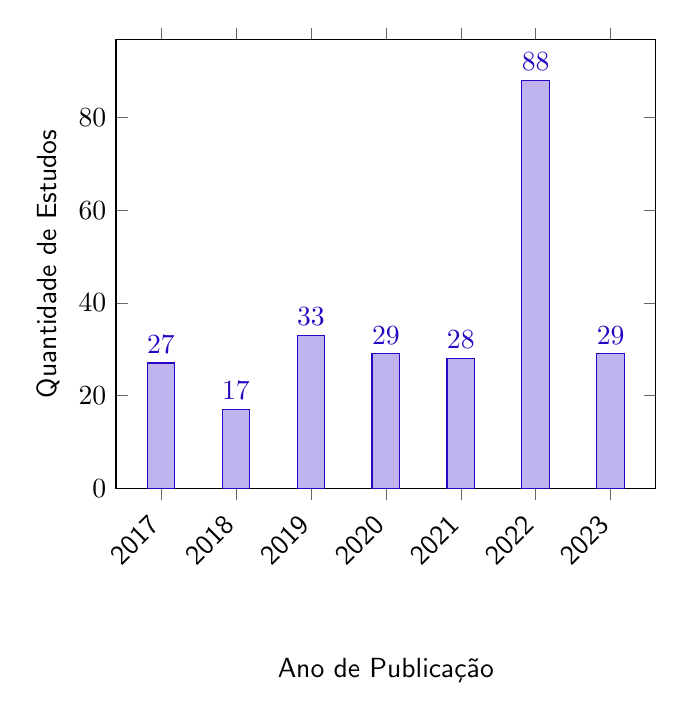
\begin{tikzpicture}
        \begin{axis}[
            ybar,
            symbolic x coords={2017, 2018, 2019, 2020, 2021, 2022, 2023},
            xtick=data,
            ymin=0,
            ylabel={Quantidade de Estudos},
            xlabel={Ano de Publicação},
            xlabel style={yshift=-25pt}, % Move o rótulo do eixo X para baixo
            nodes near coords,
            bar width=10pt, % Aumenta a largura das barras
            enlarge x limits=0.1, % Aumenta o espaçamento entre as barras
            xticklabel style={yshift=-5pt, rotate=45, anchor=east} % Rotaciona e desloca os rótulos do eixo X
        ]
        \addplot coordinates {(2017,27) (2018,17) (2019,33) (2020,29) (2021,28) (2022,88) (2023,29)};
        \end{axis}
    \end{tikzpicture}
    \\
        \centering Fonte: O autor (2024).
\end{figure}


\section{Escolha dos estudos}

Inicialmente foi realizada uma seleção preliminar analisando o título e resumos dos artigos, excluindo inicialmente estudos que não haviam relação com a temática proposta na revisão, resultando em 79 potenciais estudos a serem analisados. Após essa etapa preliminar, foi realizada a filtragem através dos Critérios de Inclusão e Exclusão citados abaixo.

\par\vspace{1\baselineskip}

\textbf{Critérios de inclusão}
\begin{itemize}
    \item CI-1: Pesquisas que tratam da inovação social aberta;
    \item CI-2: Pesquisas que tragam práticas realizadas por meio de universidades;
    \item CI-3: Pesquisas que são estudos primários.
\end{itemize}

\par\vspace{1\baselineskip}

\textbf{Critérios de exclusão}
\begin{itemize}
    \item CE-1: Pesquisas que não tratam do tema da inovação social aberta;
    \item CE-2: Pesquisas que não tenham sido realizadas no âmbito universitário;
    \item CE-3: Pesquisas que não são estudos primários (Resumos, resenhas, apresentações, e afins).
\end{itemize}

Dentre os 79 pré-selecionados, 22 foram removidos por serem não-primários (CE-3), e 46 por não tratarem da temática de inovação social aberta (CE-1) e/ou por não serem realizados no âmbito universitário (CE-2). 

O total de artigos que atenderam os três critérios de inclusão foi de 11 artigos.

\begin{table}[H]
\centering
\caption{Apresentação do quantitativo de estudos totais e selecionados}
\begin{tabular}{cccc}
\rowcolor[HTML]{C0C0C0} 
\textbf{Base de dados} & \textbf{Total} & \textbf{Selecionado} & \textbf{\%} \\
IEEE                   & 251            & 11                   & 4,38\%      \\
SBC/SOL                & 0              & 0                    & 0\%        
\end{tabular}
\vspace{0.2cm}

{\centering Fonte: O autor (2024). \par}
\end{table}




Os artigos foram publicados por pesquisadores de universidades dos seguintes países: EUA, Portugal e Tailândia com dois artigos cada e Africa do Sul, Brasil, China, Noruega, Sri Lanka, e Taiwan, possuem somente um artigo cada.

\section{Direcionamento dos Artigos}

Ao realizar uma leitura profunda e observação de cada um dos artigos, é possível observar através de seus objetivos, o direcionamento de cada artigo, como demonstrado na tabela abaixo.

\begin{table}[H]
\centering
\caption{Classificação dos estudos}
\begin{tabular}{cc}
\rowcolor[HTML]{C0C0C0} 
\textbf{Classificação}  & \textbf{Quantidade} \\
Relato de experiência   & 7                   \\
Proposta de metodologia & 4                   
\end{tabular}
\vspace{0.2cm}

{\centering Fonte: O autor (2024). \par}
\end{table}


\section{Resposta as perguntas da Revisão}

Para facilitar a compreensão do atual panorama da literatura, essa subseção irá apresentar a resposta para as perguntas da revisão, conforme os artigos selecionados.

\subsection{P1: como a universidade auxilia na prática da Inovação Social Aberta?}

Todos os artigos selecionados tratam da forma a qual a universidade realiza práticas de inovação social. O artigo S001 relata que a Universidade praticou a inovação social através da Aprendizagem de Serviço, que combina serviço comunitário voluntário e o aprendizado acadêmico, possibilitando a exploração de problemas existentes na comunidade e sua resolução através da experiência acadêmica, unindo a teoria e a prática. 

O artigo S003 utilizou a Filosofia da Economia de Suficiência (SEP), um modelo de desenvolvimento sustentável através da autossuficiência, capacitando a comunidade para atuação, auxiliando a identificação dos problemas e os dados, e a implementação de soluções viáveis pela própria comunidade. 

Já os artigos S002, S004, S007, S008 e S009 também trazem a dinâmica da universidade fornecendo capital humano e/ou material, pesquisa e desenvolvimento, suporte técnico, capacitação e formação de competências. Já os artigos S006 e S010 relatam construir soluções por parcerias entre as universidades, empresas e órgãos governamentais.  

No artigo S011, as práticas inovativas sociais ocorrem através do ensino ativo, que coloca os estudantes no centro do processo de aprendizado, estimulando também a interação entre estes e os grupos vulneráveis que irão realizar a inovação social, de fato. 

O artigo S005 evidencia a Universidade fornecendo \textit{frameworks} que promovem a criação de soluções para problemas urbanos colaborativamente entre a universidade, a administração pública e os cidadãos.

A análise dos artigos revela que, geralmente, a universidade atua como principal força motriz da realização da Inovação Social, e agindo como uma capacitadora, realizando a Inovação Aberta de dentro para fora, como pontuado por Chesbrough 2014), uma inovação que a organização abre seu processo para servir de entrada para outras organizações, praticando de forma tímida a inovação aberta de fora para dentro, onde no caso, a Universidade receberia \textit{inputs} da comunidade onde está atuando e a inovação acoplada, onde a cocriação, como um de seus principais métodos, permitiria que a criação de soluções em conjunto entre a comunidade e a universidade. 

Outro cenário observado é onde a universidade atua através parcerias com instituições, órgãos governamentais e afins, não proporcionando em sua plenitude as criações colaborativas através da Inovação Aberta acoplada. O cenário da prática da inovação social aberta em sua plenitude, através do processo de fato colaborativo, demonstrando assim, que a prática da Inovação Social Aberta encontra-se pouco difundida na academia. Os números podem ser verificados na sumarização na tabela abaixo:

\begin{table}[H]
\centering
\caption{Classificação quanto à forma da prática da Inovação Social Aberta}
\begin{tabular}{ccc}
\rowcolor[HTML]{C0C0C0} 
\textbf{Classificação}  & \textbf{Artigos}             & \textbf{Quantidade} \\
Universidade "facilitadora"  &  \begin{tabular}[c]{@{}c@{}}S002, S004, S007\\  S008, S009\end{tabular} & 5                   \\
Processos colaborativos & S001, S003, S005, S011       & 4                   \\
Parcerias entre órgãos  & S006, S010                   & 2                   
\end{tabular}
\vspace{0.2cm}

{\centering Fonte: O autor (2024). \par}
\end{table}



\subsection{P2: quais os mecanismos de colaboração entre a universidade e a sociedade?} \cite{brunswicker2018}

O artigo S001 destaca o mecanismo de colaboração entre a universidade, empresas e a comunidade, no qual os alunos atuaram diretamente com as empresas patrocinadoras e as organizações comunitárias. Semelhantemente, o artigo S002 aborda a cocriação de um \textit{Makerspace}, um espaço dedicado à cultura criativa e o desenvolvimento colaborativo. 

O artigo S003 descreve a criação de um curso pela Universidade que permite a interação direta entre alunos, facilitadores e \textit{stakeholders} externos. Da mesma forma, o artigo S010 apresenta a criação de Laboratórios de Vivência Urbana, onde a comunidade, a universidade e o governo trabalham em conjunto na cocriação de soluções urbanas segundo a necessidade da sociedade. 

Os artigos S004, S005, S006 e S007, S008, S009 E S011 enfatizam criar ecossistemas colaborativos mediante parcerias com empresas, órgãos públicos e a comunidade. 

O cenário se assemelha às conclusões da P1. Seguindo o conceito de modelos de inovação aberta de \citeauthor{brunswicker2018} (\citeyear{brunswicker2018}), é possível notar que a Universidade atua majoritariamente por meio de parcerias, para a colaboração. As principais iniciativas que representam a totalidade da Inovação Aberta tratam da criação de laboratórios e espaços de vivência, onde a universidade, a sociedade e o governo podem pensar e cocriar inovações e soluções. Além disso, existe um caso de criação de cursos que promovem a Inovação Social Aberta. Os números podem ser verificados na sumarização na tabela abaixo:
 

\begin{table}[H]
\centering
\caption{Classificação quanto aos mecanismos de colaboração universidade/sociedade}
\begin{tabular}{ccc}
\rowcolor[HTML]{C0C0C0} 
\textbf{Classificação}                                                              & \textbf{Artigos}                             & \textbf{Quantidade} \\
\begin{tabular}[c]{@{}c@{}}Parcerias bilaterais\\\end{tabular} & \begin{tabular}[c]{@{}c@{}}S001, S003, S004, S006 \\ S009, S010\end{tabular} & 8                   \\
Concursos e torneios                                                                  & S005, S008                                                                               & 2                   \\
Comunidades e redes                                                                & S008, S011                                                                               & 2                   \\
Intermediários de inovação                                                                 & S007                                                                                     & 1                  
\end{tabular}

\vspace{0.2cm}

{\centering Fonte: O autor (2024). \par}
\end{table}



\subsection{P3: como a extensão universitária faz parte dessa colaboração?}

A cultura de extensão universitária é algo que pode variar de país para país. Esse conceito é muito característico das universidades brasileiras, e pode ser chamado por outros nomes em outros países, como \textit{University Outreach}. Dos 11 artigos, somente um é brasileiro. Apesar da extensão não ser mencionada, as atividades de todos os artigos selecionados possuem a natureza extensionista de colaboração, que se materializa na troca de saberes entre universidade e sociedade (através da interação dialógica), além do impacto gerado na formação do estudante e também na sociedade.


\subsection{P4: quais as evidências e dificuldades acerca da extensão universitária nesse processo?}

O artigo S001 destaca como principais pontos melhoria: maior desempenho acadêmico dos alunos, desenvolvimento de habilidades e criação de conexões com empregadores, porém, aponta como desafios a necessidade de financiamento, dificuldade no engajamento de parceiros a longo prazo, e dependência de apoio contínuo para prosseguimento do projeto. Da mesma forma, o artigo S002 menciona como pontos positivos: aumento da confiança dos participantes, desenvolvimento de habilidades técnicas e mudança de percepção sobre a capacidade dos participantes. Os desafios foram a manutenção do engajamento, superação das barreiras sociais e sustentabilidade financeira do projeto. 

O artigo S003 ressalta o sucesso no novo sistema de abastecimento de água, que teve seu êxito em decorrência do envolvimento e colaboração entre universidade, governo e comunidade, e destaca como dificuldades a necessidade de manutenção contínua e sustentabilidade financeira do projeto. Já o artigo S004 aponta que a abordagem utilizada melhorou o engajamento e criatividade dos participantes, porém, enfrentou como dificuldades a limitação de tempo para a colaboração, dificuldades no uso das plataformas digital e problemas de envolvimento dos stakeholders. O artigo S005 apresenta como pontos positivos o envolvimento acadêmico, mas aponta como desafio a motivação da participação contínua dos cidadãos. 

No contexto do desenvolvimento profissional, o artigo S006 apresenta como pontos positivos o desenvolvimento da indústria local e capacitação dos profissionais, porém, aponta como dificuldades a falta de tecnologia para os trabalhadores locais. O artigo S007 cita que os principais desafios foram a falta de colaboração entre a universidade e a sociedade. Já o artigo S008 menciona o financiamento do projeto e sua viabilidade econômica como seus principais desafios.

Os artigos S009 e S010 tratam de questões sobre comunicação e implementação dos projetos. O artigo S009 destaca as dificuldades de comunicação e colaboração entre a universidade e as empresas, pois, a pesquisa acadêmica muitas vezes não é facilmente compreendida pelas empresas. Também é mencionada as dificuldades de financiamento do projeto e resistência a mudança dos \textit{stakeholders} citados no artigo. Já o artigo S010 ressalta como dificuldades a necessidade de adaptação das metodologias acadêmicas para o contexto prático, a dificuldade do engajamento contínuo e a dependência de financiamento.

O artigo S011 destaca como melhorias: aumento da motivação e criação da inovação. No entanto, menciona como desafios a adaptação das metodologias acadêmicas para o contexto prático, além da dependência de financiamento. 

É possível observar que, na maioria nos artigos, a dificuldade é da sustentabilidade financeira do projeto, pois, em decorrência dos projetos serem realizados no âmbito universitário, necessitam de investimentos externos a universidade. Em seguida, é o envolvimento/engajamento dos participantes. Outro ponto relatado em diversos artigos, é a facilitação dos conteúdos acadêmicos para o contexto prático, com atores fora da academia e também a resistência a mudança de alguns setores da sociedade com as inovações propostas e construídas. Um artigo relatou como dificuldade a falta da comunicação entre as partes envolvidas no projeto. Os números podem ser verificados na sumarização na tabela abaixo:


\begin{table}[H]
\centering
\caption{Classificação conforme as evidências e dificuldades relacionadas à extensão universitária}
\begin{tabular}{ccc}
\rowcolor[HTML]{C0C0C0} 
\textbf{Classificação}                                                       & \textbf{Artigos}                       & \textbf{Quantidade} \\
\begin{tabular}[c]{@{}c@{}}Sustentabilidade\\ financeira\end{tabular}        & \begin{tabular}[c]{@{}c@{}}S001, S002, S003, S008,\\ S009, S010, S011\end{tabular} & 7                   \\
\begin{tabular}[c]{@{}c@{}}Dificuldades de\\ engajamento\end{tabular}        & \begin{tabular}[c]{@{}c@{}}S001, S002, S004,\\  S005, S009, S010\end{tabular}      & 6                   \\
\begin{tabular}[c]{@{}c@{}}Adaptação\\ dos métodos\\ acadêmicos\end{tabular} & S010, S011                                                                         & 2                   \\
\begin{tabular}[c]{@{}c@{}}Resistência a\\ mudança\end{tabular}              & S009, S010                                                                         & 2                   \\
\begin{tabular}[c]{@{}c@{}}Problemas de\\ comunicação\end{tabular}           & S007                                                                               & 1                   
\end{tabular}
\vspace{0.2cm}

{\centering Fonte: O autor (2024). \par}
\end{table}


\section{Considerações finais da Revisão}

O quantitativo de artigos demonstra a carência da literatura acerca do trabalho da Inovação Social Aberta praticada no âmbito das universidades, e justifica a necessidade deste trabalho. O quantitativo de artigos publicados por brasileiros demonstra que este tema aparenta ser pouco explorado pela academia no país. As perguntas também pontuam que as maiores dificuldades nos projetos de Inovação Social Aberta são a falta de investimento, a dificuldade no engajamento das partes e resistência a mudança por parte dos setores da sociedade. E que os ganhos das práticas são benéficos tanto para a sociedade, que possui seu problema solucionado, quanto para a universidade, que consegue estreitar os laços com a sociedade, além de preparar melhor seus estudantes para a resolução de problemas. Os artigos selecionados demonstram as formas de colaboração existentes entre a universidade e a sociedade, e quais são os principais êxitos e dificuldades que foram encontradas ao longo deste processo colaborativo, mostrando também a forma que a universidade apoia e incentiva estas práticas de Inovação Social Aberta, além dos impactos gerados pelas mesmas.
  
  \chapter{Metodologia}
\label{chap:metodologia}

Este capítulo visa apresentar a metodologia que será empregada na realização desse trabalho, visando atender seus objetivos gerais e específicos.

\section{CARACTERIZAÇÃO DA PESQUISA}
Segundo \citeauthor{wazlawick2014} (\citeyear{wazlawick2014}), a área da Ciência da Computação é normalmente classificada como parte das ciências exatas ou das engenharias, mas diversas subáreas da computação estão mais próximas das ciências sociais. Este trabalho de mestrado irá realizar um estudo de caso, por meio de diagnóstico, documentação e formalização do projeto de extensão CInbora Impactar (\href{https://sigaa.ufpe.br/sigaa/link/public/extensao/visualizacaoAcaoExtensao/1971}{\textit{Link} com detalhes do projeto}), e a realização de práticas de pesquisa-ação em um projeto de Extensão utilizando a Inovação Social Aberta.

As pesquisas científicas, segundo, \citeauthor{wazlawick2014} (\citeyear{wazlawick2014}, pp. 41-42) podem ser classificadas a respeito da sua natureza, como um resumo de assunto, que versa somente sobre a sistematização de uma área de conhecimento, mostrando sua evolução ao longo do tempo, e como se encontra atualmente o estado da arte ou um trabalho original, que apresenta melhorias para teorias existentes ou até mesmo a proposição de novas teorias, para avançar o estado da arte da ciência.

Elas também podem ser classificadas quanto a seus objetivos (\citeauthor{gil2002}, \citeyear{gil2002}, pp. 41-42), como pesquisas exploratórias, descritivas ou explicativas. Na pesquisa exploratória o autor irá examinar uma série de fenômenos e variáveis buscando maior familiaridade com o problema, tornando-o mais concreto, e criando hipóteses acerca deste. Já na descritiva os fatos serão abordados como o são, através da descrição das características do objeto a ser estudado. E a pesquisa explicativa, além de analisar os dados, irá buscar responder às causas desses dados e suas explicações.

Uma terceira classificação trazida por \citeauthor{wazlawick2014} (\citeyear{wazlawick2014}, pp. 21-24) versa acerca dos procedimentos técnicos que serão realizados na pesquisa, que podem ser classificados por Pesquisa bibliográfica, documental, experimental, de levantamento ou pesquisa-ação. A pesquisa bibliográfica é um dos primeiros passos e visa o estudo de materiais científicos que já foram publicados anteriormente a respeito de determinado tema. Já a pesquisa documental analisa documentos, relatórios, normas, bancos de dados, e outros, que não estão disponíveis de forma sistematizada. A pesquisa experimental realiza tentativas experimentais através da manipulação de variáveis e/ou fatores por parte do pesquisador para observar os resultados dos mesmos. A pesquisa de levantamento busca dados a respeito do ambiente, de comportamentos, das pessoas inseridas nele, por meio de questionários, \textit{surveys}, e afins. E na pesquisa-ação o pesquisador interage diretamente com aqueles que estão sendo os objetos da pesquisa, visando promover mudanças e geração de conhecimento, unindo assim, a prática com a teoria.

\citeauthor{creswell2007} (\citeyear{creswell2007}, p. 27) traz também três métodos de pesquisa, sendo conjuntos de procedimentos a serem adotados para coleta, análise e interpretação de dados, e são os métodos quantitativos, qualitativos e mistos. Nos métodos quantitativos o pesquisador utiliza de estratégias e técnicas de pesquisa como levantamento e experimentos para gerar dados estatísticos que permitam sua observação e mensuração Os métodos qualitativos utilizam de estratégias mais voltadas para a observação de comportamento e do ponto de vista dos participantes da pesquisa sobre os fenômenos estudados, por meio de fenomenologia, etnografia, estudo de casos, e outros. E os métodos mistos empregam o uso das duas abordagens em conjunto.

Essa proposta de trabalho classifica-se como:

\begin{quadro}[H]
\caption{Classificação metodológica da proposta de trabalho}
\centering
\begin{tabular}{|
>{\columncolor[HTML]{9B9B9B}}l |l|}
\hline
\textbf{Método de Pesquisa}      & Pesquisa Qualitativa                                                                                                \\ \hline
\textbf{Natureza}      & Trabalho Original                                                                                                             \\ \hline
\textbf{Objetivos}     & Exploratório e descritivo                                                                                                     \\ \hline
\textbf{Procedimentos} & \begin{tabular}[c]{@{}l@{}}Revisão rápida de literatura, \\estudo de caso e pesquisa-ação.\end{tabular} \\ \hline
\end{tabular}
\vspace{0.2cm}

{\centering Fonte: O autor (2024). \par}
\end{quadro}

\section{DESENHO DA PESQUISA}
\label{desenhodepesquisa}

Segundo \citeauthor{marconi2003} (\citeyear{marconi2003}), o desenvolvimento de um projeto de pesquisa compreende seis passos: 
“Seleção do tópico ou problema para a investigação, definição e diferenciação do problema, levantamento de hipóteses de trabalho, coleta, sistematização e classificação dos dados, análise e interpretação dos dados e relatório do resultado da pesquisa”.

Esses passos podem ser agrupados em quatro fases: preparação de pesquisa, fases da pesquisa, execução da pesquisa e relatório de pesquisa. A preparação de pesquisa será desconsiderada aqui, por envolver escolha do tema, constituição de equipe de trabalho, cronograma e outros. \cite{marconi2003}


Na etapa de Fases da pesquisa, serão tratados: a escolha do problema que será investigado, a definição deste, e o levantamento das hipóteses acerca do problema. Essa etapa irá envolver:
\begin{itemize}
    \item \textbf{Revisão rápida de literatura}: visa observar o atual panorama da inovação social aberta praticada pelas universidades em instituições do terceiro setor nas principais bases de dados da área da ciência da computação, através da metodologia de revisão rápida proposta por \citeauthor{cartaxo2020} (\citeyear{cartaxo2020});
    \item \textbf{Identificação dos principais atores:} como a inovação social aberta envolve diferentes instituições, e por consequência, uma gama de diferentes atores, deverão ser identificados quais os principais que deverão ser observados com uma maior atenção, e que poderão proporcionar \textit{feedbacks} posteriores a equipe de pesquisa sobre os métodos propostos.
    \item \textbf{Criação do protocolo de entrevistas, grupos focais e formulários}: para colher os \textit{feedbacks} dos principais atores envolvidos, serão criadas estratégias de entrevistas, grupos focais e formulários com os participantes. Essas entrevistas deverão ser validadas anteriormente pela equipe de pesquisa, antes de serem aplicadas.
\end{itemize}

Na etapa de Execução da pesquisa será realizada a coleta e análise de dados, a criação do processo e validação, que envolverá: 
\begin{itemize}
    \item \textbf{Realização das entrevistas, grupos focais e formulários:} realização do que foi concebido na etapa anterior;
    \item \textbf{Análise das entrevistas, grupos focais e formulários}: serão analisadas as entrevistas, grupos focais e formulários, além de todas as questões colocadas pelos entrevistados;
    \item \textbf{Criação do processo para projeto de extensão}: a criação do projeto de Extensão utilizando a Inovação Social Aberta no terceiro setor, após observar os \textit{feedbacks} colhidos nas entrevistas;
    \item \textbf{Validação do processo para projeto de extensão}: o processo proposto será validado durante sua execução, e os \textit{feedbacks} serão coletados durante a análise de dados, que podem ocorrer diversas vezes.
\end{itemize}

A etapa de Relatório de pesquisa trará os resultados obtidos através da pesquisa, suas conclusões e metodologia utilizada. Essa última etapa é a publicização do que foi realizado em toda a pesquisa, e consiste em:
\begin{itemize}
    \item \textbf{Sintetização dos resultados obtidos}: A exposição de todo o conhecimento obtido com os dados trabalhados durante a pesquisa;
    \item \textbf{Confecção da Dissertação}: Escrita da dissertação de mestrado;
    \item \textbf{Apresentação do trabalho}: Apresentar uma sumarização de toda a pesquisa para a banca;
    \item \textbf{Correções finais}: realizar correções na dissertação conforme as orientações da banca.
\end{itemize}

A pesquisa será realizada em ciclos iterativos, visando o incremento das sugestões de melhorias propostas pelos \textit{stakeholders} no processo ao longo da sua execução. Por conta disso, algumas etapas serão provavelmente realizadas mais de uma vez. Esses passos são necessários para garantir o procedimento e o tratamento científico exigido pelo trabalho. Para facilitar a compreensão da forma como a pesquisa se desenvolverá, a figura abaixo traz uma síntese do desenho da pesquisa:

\input{images/metodologia/desenhodepesquisa}



\section{Plano de Pesquisa-Ação}
\label{pesquisaacao}

Segundo \citeauthor{tripp2005} (\citeyear{tripp2005}), a pesquisa-ação é uma forma de investigação-ação que utiliza as técnicas já consagradas da pesquisa científica por meio de ações tomadas para a melhoria da prática. Possui as fases de: Planejamento, implementação e avaliação, e essas fases ocorrem tanto para a parte da pesquisa (teórica) quanto a parte da ação (prática), e serão produzidos dados sobre os efeitos ocorridos advindos das mudanças empregadas.

A pesquisa-ação a ser realizada possuirá como universo o projeto de extensão CInbora Impactar, coordenador pelo Professor Kiev Gama. Esse projeto é uma iniciativa que visa promover a interação entre a \gls{UFPE} e a comunidade por meio da colaboração com o Projeto Bora Impactar \url{https://www.instagram.com/boraimpactarrecife/}, da Secretaria de Ciência, Tecnologia e Inovação da Prefeitura do Recife, possibilitando o desenvolvimento de soluções de software que atendam às necessidades de \gls{ONG}s do Recife, e também o projeto de extensão CInovação Social, coordenado pelo estudante Pedro Rodolfo e pelo Professor Kiev Gama, em parceria com a ONG Gris Social \url{https://www.instagram.com/gris.solidario/}, que busca a promoção da interação entre a \gls{UFPE} e o terceiro setor, de uma forma direta, não possuindo um intermediário como o projeto CInbora Impactar, visando uma relação dialógica, de troca de saberes.

\par\vspace{1\baselineskip}

\input{images/metodologia/partesenvolvidas}

Baseado no ciclo de pesquisa-ação de \citeauthor{staron2020} (\citeyear{staron2020}), o plano de pesquisa-ação, proposto nesse trabalho, constitui-se de 5 fases num período de 5 meses, como mostrado na imagem abaixo:

\input{images/metodologia/pesquisaacao}


\textbf{1. Diagnóstico — 4 semanas de duração}

Nessa seção, o atual planejamento e metodologias de execução do projeto por parte do professor serão analisados, além de uma identificação inicial das oportunidades de melhoria, focando na interação maior entre os envolvidos, possibilitando um maior processo de inovação aberta. 
Ações: 
\begin{itemize}
\item Realização de entrevistas com os estudantes e o professor acerca do que é esperado para o projeto, sua execução e seus resultados. 
\par\vspace{1\baselineskip}

\end{itemize}

\textbf{2. Plano de ação — 4 semanas de duração}

Será realizado um plano de projeto de Extensão, utilizando práticas já existentes de Inovação Social Aberta. 
Ações:
\begin{itemize}
    \item Levantamento de atores envolvidos;
    \item Criação de proposta de atividades para promover a colaboração entre os atores;
    \item Criação de cronograma proposto para intervenção.
\par\vspace{1\baselineskip}

\end{itemize}

\textbf{3. Tomada de ação —  4 semanas de duração}

Essa fase irá ser executada em uma interação mais direta com o professor e os estudantes, enquanto os mesmos estão trabalhando no processo de construção do artefato que será apresentado posteriormente. Ações:
\begin{itemize}
    \item Monitoramento do impacto sobre os \textit{stakeholders} envolvidos a respeito da execução do projeto
\par\vspace{1\baselineskip}

\end{itemize}

\textbf{4. Avaliação — 4 semanas de duração}

Essa etapa irá verificar se de fato as ações propostas causaram algum impacto sobre os atores envolvidos, e também nos artefatos produzidos pelos estudantes. Ações:
\begin{itemize}
    \item Análise do processo de pesquisa-ação até o momento;
    \item Análise dos artefatos produzidos pelos estudantes;
    \item Grupos focais e formulários com os envolvidos, sobre o processo de interação e colaboração entre os envolvidos;
    \item Identificação de possíveis melhorias.
\par\vspace{1\baselineskip}

\end{itemize}

\textbf{5. Aprendizado — 4 semanas de duração}

Nessa última fase será documentado todo o aprendizado obtido ao longo da execução da pesquisa-ação, e construção do possível processo a ser proposto. Ações:
\begin{itemize}
    \item Documentação das lições aprendidas;
    \item Documentação dos possíveis pontos de melhoria;
    \item Documentação dos impactos sobre todos os envolvidos e sobre o projeto.
\end{itemize}



\section{Análise de Dados}
\label{analisededados}

A análise dos dados será realizado através dos seguintes passos:

\begin{itemize}
    \item \textbf{Transcrição}: Todas as entrevistas e grupos focais serão transcritos por meio de Inteligência Artificial, e serão posteriormente revisadas pelos pesquisadores, a fim de garantir fidelidade à fala dos participantes.
    \item \textbf{Organização dos dados:} Atribuição das falas a cada um dos entrevistados e posterior anonimização das falas, substituindo nomes por pseudônimos ou códigos e armazenamento seguro dos dados obtidos, e organização separada dos grupos focais e entrevistas. Em segunda execução, foi realizada análise de dados de entrevistas e grupos focais com os estudantes e colaboradores da ONG que foi aplicado o projeto de extensão. 
    \item \textbf{Análise de Conteúdo:} Será aplicada a Análise de Conteúdo de acordo com \citeauthor{bardin2011} (\citeyear{bardin2011}):
	\begin{itemize}
	    \item \textbf{Pré-análise:} Identificação das categorias consoante as falas dos participantes;
	\item \textbf{Exploração do material:} Codificação, classificação e agregação para agrupamento de falas com temas semelhantes para identificar possíveis padrões, por meio de ferramentas de análise;
	\item \textbf{Tratamento dos resultados:} inferência e interpretação dos dados obtidos e tratados.
	\end{itemize}


\end{itemize}

\subsection{Aspectos Éticos}
O projeto de pesquisa foi aprovado no Comitê de Ética em Pesquisa da \gls{UFPE}, com o Certificado de Apresentação de Apreciação Ética de n.º 87185225.7.0000.5208, contendo detalhes da Metodologia, Métodos de Recrutamento de Participantes, Critérios de Inclusão e Exclusão, Riscos e mitigação, dentre outras informações pertinentes. Todos os participantes da pesquisa assinaram um Termo de Consentimento Livre e Esclarecido. O modelo deste termo encontra-se no Apêndice B. Os demais Termos utilizados possuem apenas mudanças pontuais conforme o perfil dos participantes (Estudantes, profissionais da prefeitura e colaboradores da ONG), além do termo do formulário \textit{online}.

\subsection{Produto final}

Como produto técnico deste presente mestrado profissional, será desenvolvido um Guia básico de boas práticas para a aplicação da Inovação Social Aberta (ISA) em projetos de Extensão Universitária, a partir da sistematização dos dados obtidos durante o ciclo de pesquisa-ação, nos projetos CInbora Impactar e CInovação Social. Nestes projetos, serão analisados tanto a percepção dos estudantes quanto dos envolvidos das instituições parceiras, sobre sua vivência no projeto, os acertos e desafios metodológicos, estratégias de engajamento, e comunicação entre universidade e instituições parceiras.

Esse guia é destinado a docentes, discentes e gestores de organizações do terceiro setor, e visa fornecer orientações práticas, replicáveis e adaptáveis para equipes extensionistas que possuem interesse na implementação de ações colaborativas e dialógicas no campo da Inovação Social Aberta, voltada para a concepção de artefatos digitais como meio de transformação social.

\section{PROJETO DE EXTENSÃO CINOVAÇÃO SOCIAL}
\label{cinovacaosocial}

O projeto CInovação Social foi concebido visando a prática da Inovação Social Aberta por meio da Extensão Universitária, voltado para estudantes do curso de Sistemas de Informação do \gls{CIn}/\gls{UFPE}, em parceria com uma \gls{ONG}, no caso de sua primeira execução, com a GRIS Solidário.

A organização se situa no bairro da Várzea, e o seu cerne é o atendimento e apoio lúdico-pedagógico para crianças em situação de vulnerabilidade social e também às suas mães, porém também possui uma forte atuação em pautas acerca de conscientização e enfrentamento ao racismo ambiental.

A escolha de atuação com uma \gls{ONG} se deu ao fato do dado apontado por Gama, que relata que ONGs possuem poucos recursos humanos e financeiros para executarem exitosamente suas atividades inovativas. E a escolha em particular da GRIS Solidária se deu em decorrência de sua proximidade com a \gls{UFPE}, visando facilitar a vivência dos espaços da ONG presencialmente pelos estudantes que irão atuar no projeto de extensão.

Apesar de ser um projeto voltado para a concepção de artefatos digitais por meio da computação, o principal foco do projeto versa sobre as pessoas que estão envolvidas nele, e todo o impacto que pode ser gerado pela relação dialógica entre os estudantes e a sociedade.

A metodologia vivenciada no projeto é uma adaptação da \textit{Speedplay} de Maria Ângela Ferrario, que preconiza a concepção de artefatos digitais como veículos de mudança social. É voltada para comunidades que possuem um difícil acesso pelo poder público e que necessitem de soluções que sejam realizadas num espaço de tempo reduzido, dispondo de metodologias ágeis para essa finalidade.

No caso do CInovação Social, o artefato digital construído foi uma Aplicação \textit{Web}, que pode ser utilizada pela ONG tanto por computadores quanto por dispositivos móveis, como solicitado pela própria organização, em decorrência de nem todos os seus colaboradores possuírem acesso fácil a computadores de mesa.

Junto a metodologia \textit{Speedplay} foi adotado o \textit{Vibecoding}, ou programação via \gls{IA}, na qual os estudantes utilizaram algumas ferramentas para gerar as páginas que compõe o núcleo do projeto, e ao longo do desenvolvimento foram incrementando via programação tradicional novas funcionalidades e detalhes ao artefato digital. A utilização de \gls{IA} visa gerar no projeto uma cultura de curadoria de soluções, não apenas programação, levando os esforços dos seus participantes para um maior foco em lógica e propósito da equipe.

Apesar do desenvolvimento ser realizado em conjunto com tecnologias de \gls{IA}, durante o projeto foi amplamente ressaltada a importância da utilização destas tecnologias de forma responsável, através das seguintes orientações:
\begin{itemize}
    \item Revisão do código gerado;
    \item Utilização de \gls{IA} de forma ética;
    \item Combinação do uso de \gls{IA} com boas práticas de engenharia de software;
    \item Documentação das decisões tomadas;
    \item Uso da \gls{IA} como apoio, não como substituto do pensamento.
\end{itemize}

A dinâmica do projeto se deu através da execução de cada \textit{“mini-sprint”} resultando em um pequeno protótipo a ser incrementado nas posteriores \textit{sprints}. O início do projeto deu-se via um momento de vivência dos estudantes nos espaços físicos da \gls{ONG}, que foi chamado no projeto de \textit{Ideathon}, baseado na etapa do \textit{Speedplay}, que Maria Ângela Ferrario chama de Ponto focal, que é um momento de co-criação de projeto de protótipo. No caso do CInovação Social, o \textit{Ideathon} resultou num \textit{wireframe} co-criado com a \gls{ONG}.

\input{images/metodologia/ong001}

\input{images/metodologia/ong002}


O cronograma do projeto foi o seguinte, dentro dos quatro ciclos do Speedplay:
\par\vspace{1\baselineskip}

\textbf{Ciclo 1 (Experimentação inicial)}
    \begin{itemize}
        \item Dia 17/08 –\textit{ Prompt-base}
        \item Dia 18 à 20/08 – \textit{Sprint} 1 - Início do \gls{MVP}
        \item Dia 21/08 – \textit{Sprint Review}  - Analisar primeira versão do \gls{MVP} e ajuste do \textit{backlog};
    \end{itemize}
\par\vspace{1\baselineskip}

\textbf{Ciclo 2 (Aprimoramento)}
    \begin{itemize}
        \item Dia 22/08 à 24/08 - \textit{Sprint} 2  - Refinar \gls{MVP} e aplicar as melhorias apontadas na última \textit{Sprint Review}
        \item Dia 25/08 - \textit{Sprint Review} - Verificar a aplicação das melhorias realizadas
        \item Dia 26/08 à 28/08 - \textit{Sprint} 3 - Refinamento do \gls{MVP} e adição de funcionalidades
        \item Dia 29/08 - \textit{Status Report} 1 - Verificação de atendimento de requisitos com \gls{ONG}
    \end{itemize}
\par\vspace{1\baselineskip}

\textbf{Ciclo 3 (Validação e Iteração)}
    \begin{itemize}
        \item Dia 30/08 à 01/09 - \textit{Sprint} 4 - Refinamento do \gls{MVP} e adição de funcionalidades
        \item Dia 02/09 - \textit{Sprint Review} - \textit{Feedback} acerca do \gls{MVP}
        \item Dia 03/09 à 05/09 - \textit{Sprint} 5 - Ajustes e incrementos finais
        \item Dia 06/09 - \textit{Status Report} 2 - Validação do \gls{MVP}
    \end{itemize}
\par\vspace{1\baselineskip}

\textbf{Ciclo 4 (Fechamento e Entrega)}
    \begin{itemize}
        \item Dia 07/09 à 09/09 - \textit{Sprint} 6 - Finalização do \gls{MVP} e preparação para apresentação final
        \item Dia 10/09 - \textit{Sprint Review} - Verificação de últimos ajustes finos e correções na interface
        \item Dia 11/09 à 12/09 - \textit{Sprint} final - Ajustes verificados na última SR
        \item Dia 13/09 - Apresentação final no Espaço \textit{Pitch} - \gls{CIn}/\gls{UFPE}
    \end{itemize}

O projeto contou com a participação direta de seis estudantes do curso de Sistemas de Informação, como equipe responsável pelo desenvolvimento do artefato digital, duas colaboradoras da GRIS Solidário como fonte de informação, participantes da co-criação e validação, o professor orientador auxiliando no processo metodológico e dois pesquisadores na coordenação, coordenando o processo extensionista, e realizando mentoria com os estudantes e alinhamentos necessários com a \gls{ONG}.

Apesar das datas programadas, algumas vezes, a \gls{ONG} teve uma dificuldade em manter as datas agendadas, por conta de adversidades, um quantitativo reduzido de voluntários, onde a própria coordenadora da \gls{ONG} se desdobrou diversas vezes para executar diversas tarefas diferentes na instituição.


  \chapter{Resultados}
\label{chap:resultados}

Esse capítulo visa apresentar os resultados obtidos através da realização desse trabalho, visando sintetizar os principais pontos e tópicos observados.

\section{Análise de Dados}
\label{resultadoanalise}

A análise dos dados utilizada nos dois projetos de extensão analisados (CInbora Impactar e CInovação Social), foi realizada através da Análise de Contéudo de \citeauthor{bardin2011} (\citeyear{bardin2011}). Esta escolha foi em decorrência da possibilidade de sistematização das falas e opiniões dos entrevistados, auxiliando na compreensão da visão destes acerca da experiência do processo vivenciado na extensão universitária, em especial, da relação dialógica, e da troca de saberes proporcionada pela Inovação Social Aberta.

\input{chapters/resultados/analisecinbora}




O principal resultado deste trabalho foi um Guia visando trazer práticas experimentadas de Inovação Social Aberta na Extensão Universitária voltada para a concepção de artefatos digitais como meio de transformação social. Ele é destinado a docentes, discentes e gestores de organizações do terceiro setor, e visa fornecer orientações práticas, replicáveis e adaptáveis para equipes extensionistas que possuem interesse na implementação de ações colaborativas e dialógicas neste campo, que encontra-se anexado no Apêndice F.



  \chapter{Recomendações para a prática da Inovação Social Aberta na Extensão Universitária.}
\label{chap:recomendacoes}

Essas recomendações, como resultado desta dissertação, visam trazer práticas experimentadas, replicáveis e adaptáveis de Inovação Social Aberta na Extensão Universitária, mais especificamente voltadas para a concepção de artefatos digitais como meio de transformação social. Ele é destinado a docentes, discentes e gestores de organizações do terceiro setor que possuem interesse na implementação de ações colaborativas e dialógicas. Os dados analisados para constar neste guia são de uma revisão rápida de literatura acerca da produção acadêmica relevante sobre o tema da Inovação Social Aberta praticada por meio de universidades, do Projeto de Extensão CInbora Impactar, executado durante a disciplina de Desenvolvimento de Software, do curso de Sistemas de Informação do Centro de Informática da UFPE, em parceria com a Prefeitura da Cidade do Recife e do Projeto de Extensão CInovação Social, executado com estudantes do curso de Sistemas de Informação do Centro de Informática da UFPE em parceria com a ONG Gris Solidário da Várzea, Recife–PE.

As recomendações foram organizadas agrupadamente, e na observação dos projetos foram compiladas as seguintes:

\begin{table}[H]
\centering
\caption{Recomendações para a Extensão Universitária}
\begin{tabular}{|c|p{11cm}|}
\hline
\textbf{Recomendação} & \textbf{Descrição} \\ \hline
1 & Utilizar a Inovação Social Aberta na Extensão \\ \hline
2 & Planejar o Projeto de Extensão  \\ \hline
3 & Promover escuta ativa, respeito e empatia com a instituição \\ \hline
4 & Valorizar processos de aprendizagem e desenvolvimento com \textit{soft-skills} \\ \hline
5 & Utilizar metodologias e ferramentas de comunicação \\ \hline
6 & Utilizar ferramentas de gerenciamento de tarefas \\ \hline
7 & Empregar técnicas de ideação e geração de soluções \\ \hline
8 & Desenvolver colaborativamente artefatos digitais adequadamente \\ \hline
9 & Avaliar as soluções propostas e o aproveitamento dos estudantes \\ \hline
\end{tabular}
\end{table}



\section*{\#R1 – Utilizar a Inovação Social Aberta na Extensão Universitária}

A Extensão Universitária é um importante e poderoso instrumento da universidade que possui um enorme potencial de transformação social. Entre as suas diretrizes está a Interação Dialógica, que apregoa a participação ativa e a construção conjunta de conhecimento, valorizando o diálogo entre diferentes setores da sociedade e a universidade.

Para além da função social da Extensão Universitária, a mesma também atua como uma propagandista do trabalho executado pela Universidade, onde muitas vezes pode despertar na comunidade, que não conhece profundamente a Universidade e o seu trabalho, a vontade de ingressar nas fileiras acadêmicas.

A Inovação Social Aberta pode auxiliar em todos esses processos, por ter como seu cerne a Inovação Aberta, a qual é a troca de conhecimento, através da recepção de ideias externas, exportação de ideias e cocriação para potencialização do processo inovativo, em vez da utilização exclusiva dos próprios recursos. A Inovação Social busca criar ou aprimorar ideias, práticas, serviços, dentre outros, para atender às necessidades das comunidades e proporcionar melhores condições de vida para as mesmas.

A utilização da Inovação Social Aberta para potencializar os processos extensionistas, acaba por auxiliar a universidade a fortalecer sua capacidade, em conjunto com a comunidade, de identificar, co-criar e implementar soluções inovadoras para seus problemas reais. Esse processo não auxilia apenas o cotidiano da comunidade onde a instituição está inserida, mas também reforça o papel da universidade pública para com a comunidade na qual está inserida. Esse fortalecimento é importante para demonstrar a verdadeira essência e importância das universidades públicas, principalmente em cenários de cortes orçamentários, que são recorrentes no cenário brasileiro, como apontado por \citeauthor{spannenberg2023} (\citeyear{spannenberg2023}).
\section*{\#R2 – Planejamento do Projeto}

Um bom planejamento é extremamente importante para o sucesso de qualquer projeto, especialmente em projetos de Inovação Social Aberta por meio da extensão universitária, onde existe o envolvimento de diversos atores diferentes em sua composição. Ele vai garantir a coesão de todos os atores e equipes, delimitação de objetivos, organização de cada etapa a ser executada e uma melhor assertividade no atendimento destes objetivos.

\textbf{Definição de escopo e objetivos}:
Um dos principais pontos a ser observado ao realizar o planejamento do projeto é a definição e delimitação do escopo que será atendido e dos objetivos que serão trabalhados. Como percebido no projeto CInovação Social, as instituições, ao observarem a oportunidade de construírem algo em conjunto com a universidade, pode acabar querendo expandir o escopo do projeto, o que pode acabar sendo inviável, ao depender do projeto e de sua duração. É importante que o coordenador junto com a equipe delimite antes do início da execução do mesmo o seu escopo e os seus objetivos, além dos resultados que buscam ser alcançados, sempre focando na formação dos estudantes, nos benefícios vivenciados pela instituição e no fortalecimento do processo de relação dialógica entre a universidade e a comunidade.

Com o advento da curricularização da extensão nas universidades, cada vez mais têm se oferecido disciplinas já integradas com carga horária de extensão universitária, porém, cada projeto de extensão terá sua própria dinâmica, que poderá se adequar mais a um tipo específico de configuração de extensão.

Os projetos de extensão podem ocorrer integrados a uma disciplina ou de maneira autônoma.

\textbf{Projetos integrados a disciplinas (ex.: CInbora Impactar):}
\begin{itemize}
    \item Conteúdo teórico aplicado simultaneamente.
    \item Projetos reais em vez de simulações.
    \item Maior engajamento dos estudantes na disciplina e/ou projeto.
\end{itemize}

\textbf{Pontos negativos:}
\begin{itemize}
    \item Pode competir com outras disciplinas do mesmo semestre.
    \item Um excesso de equipes pode dificultar o gerenciamento.
    \item Participação pode se tornar impessoal devido à quantidade de estudantes.
\end{itemize}

\textbf{Projetos autônomos (ex.: CInovação Social):}
\begin{itemize}
    \item Equipes menores podem gerar participação mais pessoal e empática.
    \item Tempo de duração variável, podendo incluir períodos de férias.
\end{itemize}

\textbf{Pontos negativos:}
\begin{itemize}
    \item Possível desmotivação por ausência de impacto acadêmico perceptível a curto prazo.
    \item Dificuldade no financiamento das atividades.
\end{itemize}

\textbf{Duração do projeto e carga horária:}
Cada projeto de extensão, desde sua concepção e observando os seus objetivos e resultados esperados, deve possuir sua duração delimitada pelo coordenador e equipe com base na experiência vivenciada e pela mensuração das atividades e do tempo. Alguns dos cenários possíveis são os seguintes:

\begin{itemize}
    \item \textbf{Curto prazo}: Este cenário pode ser utilizado para projetos com menos de um semestre de duração, e é mais adequado para projetos que envolvem metodologias ágeis e prototipagem rápida;
    \item \textbf{Médio prazo}: Pode ser utilizado em disciplinas, com duração de um semestre (podendo se estender a dois semestres, se for um projeto mais longo), e é um cenário mais adequado para a curricularização da extensão;
    \item \textbf{Longo prazo}: É mais indicado para projetos estruturantes, que exija uma maior necessidade de interação entre os estudantes e a instituição, e a necessidade de diversas iterações para atingir o resultado desejado.
\end{itemize}

\textbf{Delimitação das metodologias:}
Para apoiar a definição do escopo, objetivos e resultados esperados, é importante que a metodologia que será utilizada no projeto seja bem delimitada e documentada, sempre com fases claras, e quais serão os entregáveis esperados pelo projeto. Ao longo das recomendações existem metodologias e entregáveis que podem ser utilizados em projetos de extensão que visam o desenvolvimento de artefatos digitais. 




\section*{\#R3 – Realizar uma Reunião de Alinhamento Inicial}

Antes de iniciar o projeto, é importante realizar uma reunião de alinhamento para cada estudante ter ciência das atividades que serão realizadas e começar a se apropriar do projeto e de seus objetivos.

É importante que esta reunião inicial seja um rápido briefing do que será feito, visando gerar uma expectativa positiva acerca do que poderá ser desenvolvido durante o projeto, e não algo que possa afastar os estudantes por demonstrar um nível muito grande de complexidade.

Um cronograma de execução de todo o projeto deve estar muito bem definido, incluindo marcos e datas de entrega.
\section*{\#R4 – Promover Escuta Ativa e Aproximação com a Instituição}

O momento de escuta ativa é um elemento central no processo da Inovação Social Aberta. Esse momento de empatia permite que os estudantes compreendam melhor as dores, desafios e realidade do público com o qual irão trabalhar colaborativamente.

Nesse mesmo campo, a escuta ativa pode trazer uma valorização e compreensão maior por parte da instituição que trabalhará em colaboração com a universidade, potencializando a relação dialógica. Isso permite a criação de um espaço seguro de diálogo horizontal, imprescindível para a Inovação Social Aberta.

\textbf{Boas práticas:}
\begin{itemize}
    \item Local do encontro:
    \begin{itemize}
            \item Instituição parceira: fortalece a imersão e o processo de empatia;
            \item Espaços da universidade: possui uma logística mais facilitada por ser um ambiente familiar para os estudantes, mas pode enfraquecer o processo de vivência.
    \end{itemize}

    \item Metodologias do encontro:
    \begin{itemize}
            \item Hackathon: esse tipo de encontro irá enfatizar a construção de protótipos e mínimos produtos viáveis, em curtos espaços de tempo. É um momento de construção e criação. Pode facilitar na concepção rápida do protótipo, porém, pode propiciar a atuação num escopo menor, e também exige habilidades técnicas de seus participantes.
            \item Ideathon: nesse caso, existe a ênfase na concepção de ideias criativas e soluções inovadoras para problemas específicos, podendo resultar em protótipos ou não, pois seu foco não é a construção e criação, mas sim o pensamento e a conceituação, necessitando assim de outras etapas para a construção dessas soluções.
    \end{itemize}

    \item Gestão de tempo:
    \begin{itemize}
            \item Cada um dos momentos do encontro devem possuir seu tempo máximo de execução, e preferencialmente, serem cronometrados para maior controle;
            \item Importante evitar que relatos que não colaboram ativamente com o desenvolvimento do projeto desviem o foco, porém, isso deve ser feito de maneira empática e respeitosa;
    \end{itemize}
\end{itemize}

Em algumas situações, dependendo da dimensão da equipe, o processo de ideação e seleção de ideias pode ocorrer durante a escuta ativa. Nesses casos, metodologias formais tornam-se dispensáveis, sendo necessárias somente nas metodologias de levantamento e refinamento de requisitos e prototipação.

Os estudantes tendem a se sentir mais motivados e participativos quando conseguem se colocar no lugar das pessoas que passam pelas dificuldades. Alguns relatam experiências pessoais, fortalecendo laços entre si e aumentando a motivação.

\section*{\#R5 – Utilizar Metodologias e Ferramentas de Comunicação}

Um ponto extremamente importante para o bom desenvolvimento do projeto é a comunicação, tanto interna entre a equipe executora do projeto, quanto com a instituição parceira. 

Diversas ferramentas podem ser utilizadas para comunicação em projetos de extensão. As que se demonstraram efetivas são:
\begin{itemize}
    \item WhatsApp: comunicação informal e atualizações rápidas. É importante que o WhatsApp, por ser um meio de comunicação mais difundido na sociedade, seja um espaço de utilização tanto pelos estudantes quanto pela organização. Uma boa forma de delimitar isto é por meio de um grupo de WhatsApp com todos os envolvidos no projeto, porém, delimitando que aquele espaço é exclusivamente para tratar de assuntos relacionados ao projeto, para evitar discussões paralelas sem relação com a extensão.
    \item Discord: utilizado para codificação conjunta, resolução de problemas, agendamento de reuniões, enquetes e videochamadas. É um aplicativo mais específico e de mais conhecimento dos estudantes. Pode ser mais interessante para uso interno da equipe, sem envolver a instituição parceira.
\end{itemize}
\section*{\#R6 – Definir a Duração do Projeto com Metodologias Ágeis}

É imprescindível que o projeto possua as suas etapas bem definidas. A falta dessa definição pode gerar um tom de desorganização por parte do coordenador do projeto, o que pode causar ansiedade em alguns estudantes ou até mesmo desestimular os mesmos. 

Uma possível metodologia para projetos de extensão e inovação social é a metodologia Speedplay de \citeauthor{ferrario2014} (\citeyear{ferrario2014}), o qual é um método de desenvolvimento de inovação social por meio de artefatos digitais, em ambientes que exigem uma maior celeridade, além de grupos com difícil acesso, representando uma metodologia de execução rápida, que permite uma autonomia na forma organizacional para quem irá realizar a coordenação do projeto. Como possui o foco em artefatos digitais e prototipagem rápida e exige um ritmo acelerado, o Speedplay funciona bem com programação via Inteligência Artificial (Vibecoding), que será falado nos próximos capítulos, onde o Speedplay atua como bússola metodológica, enquanto o Vibecoding traduz essa bússola em código computacional. 

Um dos momentos importantes do Speedplay é o marco chamado por Ferrario de Ponto focal, onde será um momento de aceleração da colaboração e um importante momento de engajamento. As formas de execução desse ponto focal serão mais detalhadas nos próximos capítulos.

As fases do Speedplay são as seguintes:

\begin{enumerate}
    \item Preparar: \textit{ideathon} ou \textit{hackathon} como pontos focais, levantamento de requisitos, início de protótipos.
    \item Co-Criar: exploração das ideias e desenho de soluções.
    \item Construir: construção de MVP, testes e validação.
    \item Sustentar: consolidação do aprendizado e continuidade das soluções.
\end{enumerate}

Em projetos curtos, o Scrum pode ser adaptado para “mini-sprints”, exigindo encontros frequentes de \textit{Sprint Reviews} e testes de usuários.

\section*{\#R7 – Valorizar Processos de Aprendizagem e Engajamento e Desenvolvimento de Soft-Skills}

O processo de ensino-aprendizagem é uma das partes mais importantes da extensão. Muitas das vezes se existe um grande foco na solução que será entregue, mas esta solução será somente um reflexo de todo o processo de ensino-aprendizagem vivenciado tanto pelos estudantes quanto pela instituição parceira no processo de cocriação e de inovação aberta.

O processo de inovação social aberta ocorre através da troca de aprendizado e da relação dialógica:
\begin{itemize}
    \item A instituição aprende com os estudantes.
    \item Os estudantes integram teoria e prática em experiências reais e significativas.
\end{itemize}

Isso potencializa o desenvolvimento de \textit{soft-skills}, como resolução de problemas, gerenciamento de times e pensamento crítico. É importante resgatar o protagonismo estudantil, tornando os projetos autogerenciáveis. O coordenador, entretanto, deve acompanhar constantemente, garantindo que o projeto funcione e os estudantes não se sintam somente força de trabalho.

Ao usar metodologias ágeis, funções (ex.: \textit{Product Owner}, \textit{Scrum Master}) devem ser definidas desde o início, com apoio do coordenador no desenvolvimento de habilidades gerenciais. O coordenador também pode atuar diretamente na execução, incluindo a confecção do artefato digital, gerando maior engajamento e segurança nos estudantes.

O registro de todas as atividades e decisões é fundamental para auxiliar na execução do projeto e para lições aprendidas em projetos futuros.

\section*{\#R8 – Utilizar Metodologias e Ferramentas de Comunicação}

Um ponto extremamente importante para o bom desenvolvimento do projeto é a comunicação, tanto interna entre a equipe executora do projeto, quanto com a instituição parceira. 

Diversas ferramentas podem ser utilizadas para comunicação em projetos de extensão. As que se demonstraram efetivas são:
\begin{itemize}
    \item WhatsApp: comunicação informal e atualizações rápidas. É importante que o WhatsApp, por ser um meio de comunicação mais difundido na sociedade, seja um espaço de utilização tanto pelos estudantes quanto pela organização. Uma boa forma de delimitar isto é por meio de um grupo de WhatsApp com todos os envolvidos no projeto, porém, delimitando que aquele espaço é exclusivamente para tratar de assuntos relacionados ao projeto, para evitar discussões paralelas sem relação com a extensão.
    \item Discord: utilizado para codificação conjunta, resolução de problemas, agendamento de reuniões, enquetes e videochamadas. É um aplicativo mais específico e de mais conhecimento dos estudantes. Pode ser mais interessante para uso interno da equipe, sem envolver a instituição parceira.
\end{itemize}
\section*{\#R9 – Utilizar Ferramentas de Gerenciamento de Tarefas}

O gerenciamento de tarefas é fundamental para o sucesso de projetos. Um bom planejamento e gerenciamento, além de reduzir a quantidade de erros que podem ocorrer no processo e na solução final, também evita retrabalho e permite uma otimização do tempo de todos os participantes.

Essas são algumas ferramentas básicas que podem auxiliar no gerenciamento das tarefas no projeto:

\begin{itemize}
    \item Jira: especializado em gestão de projetos de software, com rastreamento de bugs e relatórios.
    \item Notion: versátil, permite bases de dados, listas de tarefas e organização visual.
    \item Trello: simples e eficaz com quadros Kanban para backlog.
\end{itemize}

Apesar do uso dessas ferramentas, muitas vezes a comunicação informal acaba predominando como principal forma de gerenciamento. Essa não é a forma ideal, visto que não permite a documentação do projeto, o que pode dificultar para a posterior avaliação dos pontos críticos, o levantamento de lições aprendidas, e a consequente melhoria nas próximas execuções do projeto.
\section*{\#R10 – Empregar Técnicas de Ideação e Geração de Soluções}

Em alguns casos, os estudantes já podem possuir experiência prévia em ideação e geração de soluções, trazendo ideias de disciplinas e \textit{ideathons}/\textit{hackathons} que já participaram anteriormente. Porém, as instituições podem não possuir a mesma familiaridade com algumas técnicas mais conhecidas. É extremamente importante que uma boa explanação e nivelamento para que todos os envolvidos possam participar ativamente, e sem receio do processo de cocriação.

Algumas metodologias que foram experimentadas nos projetos analisados:
\begin{itemize}
    \item \textbf{Mapa de empatia}: exercício dos estudantes se colocarem no lugar das pessoas atendidas pela ONG se sentem, o que elas veem e ouvem, o que falam e fazem. Isso ajuda a entender o que realmente importa para elas.
    \item \textbf{Como podemos}: essa etapa irá transformar os problemas encontrados em perguntas que começam com “Como podemos...?”, para abrir espaço para ideias criativas e soluções práticas;
    \item \textbf{\textit{Brainstorm}}: essa etapa será um estímulo para todos pensarem em muitas ideias diferentes, sem julgar. Quanto mais ideias, melhor, e depois a triagem das que são mais úteis e fáceis de fazer.
    \item \textbf{SCAMPER}: é o acrônimo de Substituitr, combinar, adaptar, modificar, propor, eliminar e reorganizar, as quais são fases que visam desenvolvimento da criatividade, analisando todos os aspectos de um produto, seu público alvo e seu mercado;
    \item \textbf{Análise de concorrentes}: mapeamento de soluções já existentes no mercado para resolução do problema, e suas vantagens e desvantagens;
    \item \textbf{Seleção de ideias}: visando considerar todas as ideias envolvidas,  votar nas ideias que têm mais impacto para a ONG e que sejam factíveis de serem feitas no tempo do projeto, assim escolhendo as que serão trabalhadas;
    \item \textbf{Histórias de Usuário}: escrever pequenas frases acerca das ideias escolhidas, que mostram quem vai usar, o que quer fazer e qual benefício espera. Isso ajuda a organizar o trabalho.
\end{itemize}

É importante também que seja realizada uma prototipagem do que será construído, visando auxiliar no processo de co-criação e principalmente do atendimento dos requisitos levantados. Também traz uma maior motivação aos estudantes e aos outros \textit{stakeholders}, ao começarem a visualizar o trabalho de fato, sendo concretizado, e podem ser feitos das seguintes formas:

\begin{itemize}
    \item \textbf{\textit{Wireframe}}: dar uma "cara" a tudo o que foi construído ao longo do processo do Ideathon, através de desenhos em papel do que foi imaginado para a interface do artefato;
    
    \item \textbf{Figma}: protótipos de maior fidelidade comparados aos anteriores, e auxiliam para melhor entendimento de como a plataforma deverá, de fato, se comportar.

\end{itemize}

Os protótipos devem ser validados com os envolvidos antes da implementação. Por conta disto, é importante que os projetos sejam demonstrados e explicados a instituição parceira, para que a mesma mostre sua opinião acerca do que está sendo construído, além de também poderem aprender com o processo que está sendo realizado para essa solução.


\section*{\#R11 – Desenvolver Artefatos Digitais adequadamente}

Segundo o preconizado pela metodologia \textit{Speedplay} de \citeauthor{ferrario2014} (\citeyear{ferrario2014}), os artefatos digitais podem ser utilizados como meio de transformação social, o qual é o foco deste trabalho. 

Existem diversas formas de construção de artefatos digitais em projetos de extensão, e as formas vivenciadas e acertadas, que ocorreram nos projetos do Centro de Informática avaliados por essas recomendações, são as seguintes:

\begin{itemize}
    \item Programação manual: os estudantes desenvolvem todos os códigos e interfaces dos artefatos digitais. Recomendado para equipes grandes e períodos de execução mais longos.
    \item Programação via Inteligência Artificial (\textit{vibecoding}): os estudantes desenvolvem códigos e interfaces por meio da inteligência artificial, realizando manualmente correções e adaptações necessárias. Recomendado para equipes menores e períodos de execução mais curtos, permitindo maior foco nas ideias, processos e entendimento da dor da instituição.
\end{itemize}

Como a forma da realização da programação manual pode se dar de diversas formas, utilizando as mais diversas metodologias e \textit{frameworks} que já estão consolidados e são bastante conhecidos pela literatura científica, este trabalho vai trazer uma nova perspectiva, que está em amplo crescimento, e trazer algumas recomendações básicas de como utilizar exitosamente, o qual é o \textit{vibecoding}.

A forma de programação por meio de Inteligência Artificial tem se mostrado em evidência, em decorrência do crescimento súbito do tema no mercado e na mídia, o que também pode ser um motivador maior para os estudantes, por terem a oportunidade de trabalharem com novas tecnologias que estão cada vez mais em evidência no cotidiano do mercado. 

Ferramentas úteis no Vibecoding:
\begin{itemize}
    \item \textbf{ChatGPT}: visando uma melhor assertividade da utilização dos créditos gratuitos disponibilizados pelo V0/Vercel, os estudantes utilizaram o ChatGPT para melhor criação do \textit{prompt} conforme os requisitos levantados em conjunto com a ONG e com a interface que foi prototipada, seja no Wireframe ou no FIGMA, onde o ChatGPT permite a adição de fotos, facilitando na construção do \textit{prompt};

    Exemplo de \textit{prompt} utilizado no projeto CInovação Social: Crie um prompt para o v0 com base nesse projeto (descrição básica do projeto) e nesse protótipo (enviado imagem do protótipo do FIGMA).
    
    \item \textbf{V0 - Vercel}: as interfaces (front-end) do projeto CInovação Social e seu banco de dados foi todo gerado via IA através do V0, onde os estudantes, através do \textit{prompt} gerado pelo ChatGPT, gerou o código em React/Next.js com Tailwind, entregando componentes reutilizáveis, e também gerando o \textit{back-end} e o banco de dados completo no Supabase, além de realizar automaticamente a integração destes 3 componentes da plataforma. Em decorrência do V0 ser pago e possuir poucos créditos gratuitos, foi utilizado para gerar o núcleo duro do artefato, onde os estudantes poderão trabalhar em cima do projeto, refinando o mesmo. O tempo economizado durante a construção dos principais componentes necessários para a solução pode ser utilizado para a documentação e melhoria incremental do projeto.
    
    \item \textbf{Gemini}: diversos erros foram ocorrendo durante o processo de criação da solução através do V0/Vercel, e para a correção dos erros, seja de interface ou do funcionamento na lógica, cada correção era cobrada a parte pela plataforma, e muitas das vezes as soluções eram incompletas, gerando mais cobranças para novas correções. Em vez de realizar as correções pelo V0/Vercel, os erros e os códigos foram enviados para o Gemini, onde o mesmo realizava a proposta de correção, que era analisada pelos estudantes e era integrada de fato no projeto. Alguns erros se repetiam em diferentes módulos do sistema, e ao corrigir algum caso específico junto ao Gemini, os estudantes conseguiram otimizar o tempo aplicando as mesmas correções em outros módulos, gerando também um aprendizado coletivo sobre padrões de erro e correções no código.
    
    \item \textbf{Copilot}: essa ferramenta foi utilizada durante o processo de codificação por parte dos estudantes, onde a correção de erros do V0/Vercel e do Gemini não foi efetiva, e precisava de um olhar mais detalhado pelos estudantes, através da utilização de ferramentas de codificação comuns como o Visual Studio Code, em auxilio do Copilot para correções mais pontuais via IA.
\end{itemize}

\section*{\#R12 – Adotar Boas Práticas de Desenvolvimento Colaborativo}

É importante garantir que boas práticas estão sendo adotadas durante o desenvolvimento colaborativo, que muitas vezes pode ser desafiador por envolver estudantes de períodos diferentes, cursos diferentes, e realidades diferentes, além do envolvimento da instituição parceira, que pode ter limitações que dificulte sua participação neste desenvolvimento.

Algumas práticas foram adotadas ao longo das execuções dos projetos analisados:
\begin{itemize}
    \item Dias fixos de trabalho: o \textit{Product Owner} do projeto pode definir dias e horários fixos para todos desenvolverem colaborativamente, evitando que o único momento de encontro entre toda a equipe seja no \textit{Sprint Review}. Isso pode auxiliar e estimular a responsabilidade dos participantes e o engajamento dos mesmos. Em casos de projetos que estão sendo executados em períodos de férias, pode se dar uma preferência aos horários já reservados para as aulas, auxiliando assim a organização dos estudantes. Em projetos executados em períodos de aula, podem ser ao fim de semana, respeitando o descanso dos estudantes. Esses encontros podem ser tanto presenciais quanto \textit{online}. O uso da ferramenta Discord no projeto CInovação Social permitiu a otimização destes momentos através dos canais de voz, onde os estudantes poderiam conversar entre si por voz, compartilhar suas telas para mostrarem o que estavam fazendo, além de poderem enviar código via chat, acelerando o processo.
    
    \item Delimitação de tarefas: deve se ter uma forte delimitação dos papéis que serão executados pelos estudantes e pelo coordenador do projeto, além dos papéis que serão exercidos pelos colaboradores da instituição parceira. Caso adotada metodologias como o Scrum, devem ser delimitados os papéis básicos como \textit{Product Owner}, \textit{Scrum Master}. Também deve haver o direcionamento e a separação de tarefas da concepção e do desenvolvimento do artefato digital, evitando sobreposição de trabalho e retrabalho entre os estudantes, além de deixar os mesmos mais confortáveis de trabalharem nas áreas que se sentem mais capacitados.

    \item Feedback contínuo: é importante que o coordenador estimule o \textit{feedback} contínuo em relação às tarefas que os estudantes estão executando ao longo do desenrolar do projeto, tanto do coordenador para com os estudantes, dos estudantes para consigo mesmos e dos estudantes para o coordenador, auxiliando na melhoria do projeto não somente em cada nova iteração, mas ao longo da própria execução do mesmo.

\end{itemize}

\section*{\#R13 – Avaliar as soluções propostas e o aproveitamento dos estudantes}

A avaliação em projetos de extensão pode ser algo complexo, pois não é um processo de mensuração tal qual uma prova de alguma disciplina. O processo de extensão toca em diversos pontos que não são tangíveis e não são avaliados por um simples barema. O processo avaliativo não deve jamais levar somente em conta a qualidade dos produtos finais, mas sim todo o processo de ensino-aprendizagem vivenciado pelos estudantes e pela instituição e a relação dialógica que se estabeleceu ao longo das vivências do projeto.

A avaliação deve ser pensada de uma forma multidimensional, e deve envolver todos os participantes do projeto, tanto os que fazem parte da universidade, quanto os que fazem parte da instituição do terceiro setor parceira e, se possível e aplicável, da comunidade ao redor.

Formas de avaliação:

\begin{itemize}
    \item \textbf{Avaliação 360:} esse tipo de avaliação permite que todos os participantes avaliem todas as partes envolvidas, tanto da universidade quanto da instituição, e por ser anônima, permite uma avaliação menos enviesada e mais sincera;
    \item \textbf{Avaliação por pares:} os estudantes podem se avaliar mutualmente ao longo da execução do projeto, estimulando a responsabilidade mútua;
    \item \textbf{Autoavaliação reflexiva:} os estudantes podem avaliar a si e atribuírem notas para cada critério, levando-os a momentos de autocrítica e de desenvolvimento de responsabilidade;
    \item \textbf{Avaliação pela instituição e/ou comunidade:} esse momento é o de verificar se as soluções propostas de fato auxiliam a resolver as problemáticas colocadas ao longo da execução do projeto, e se os principais requisitos foram atendidos.
\end{itemize}

É importante que as formas de avaliação sejam utilizadas combinadamente, auxiliando assim na efetividade do projeto. Também deve ser ressaltado para os estudantes que o processo avaliativo serve para o aprimoramento do processo extensionista, e maior assertividade em próximas execuções.











  \chapter{Considerações Finais}
\label{chap:consideracoesfinais}

Como apontado ao longo do trabalho, a literatura acerca do tema abordado é muito escassa. Essa trabalho visou preencher uma lacuna existente na literatura científica, sobre pesquisas relacionadas a Inovação Social Aberta no Terceiro Setor por meio da Extensão Universitária, além de observar e mapear quais são essas atividades, e quais são os principais desafios e sucessos.

Através das observações da literatura e dos projetos de extensão CInbora Impactar e CInovação Social já citados ao longo do texto, foi construído um Guia de Práticas em Inovação Social Aberta na Extensão Universitária, como produto técnico exigido pelo Mestrado Profissional em Ciência da Computação, baseado nas recomendações demonstradas por esta dissertação, que pode servir como referência para docentes, discentes, coordenadores de extensão e instituições do terceiro setor que possuam interesse em praticar a Inovação Social Aberta no seu contexto, através da extensão universitária.

Essa pesquisa buscou aproximar a teoria e a prática, além de contribuir com a consolidação da inovação social aberta, principalmente no meio universitário e obteve bons resultados com projetos contando com um grande engajamento por parte dos estudantes e das instituições envolvidas, além na grande qualidade dos artefatos desenvolvidos.

Para trabalhos futuros, além do fortalecimento do guia, da validação com outros projetos e de suas melhorias, também existe a possibilidade da realização de plataformas digitais que potencializem esse guia, e demonstrem de forma mais prática como \textit{toolkits}, onde os interessados poderão navegar pelo guia, ver vídeo-aulas ensinando a realizarem as práticas e as metodologias propostas, além da proposição de cursos para a utilização desta plataforma e também da disseminação da prática da Inovação Social Aberta através da Extensão Universitária, para além dos cursos do Centro de Informática, como foram observados neste projeto. 

Também podem ser realizados trabalhos de fortalecimento da curricularização da extensão universitária por meio da criação de guias e recomendações mais específicas para integração de projetos em mais de uma disciplina, através das mais variadas metodologias, como exemplo a Aprendizagem Baseada em Problemas ou Desafios.

\bookmarksetup{startatroot}% 


% ----------------------------------------------------------
% ELEMENTOS PÓS-TEXTUAIS
% ----------------------------------------------------------
\postextual


% ----------------------------------------------------------
% Referências bibliográficas
% ----------------------------------------------------------
%\bibliographystyle{abntex2/abntex2-alf.bst} %caso seja em inglês, retire o comentário desta linha
% \renewcommand{\bibname}{REFER\^ENCIAS}
%\renewcommand{\bibname}{Bibliography}
% \addbibresource{sample.bib}

\bibliography{references2.bib}


% ----------------------------------------------------------
% Apêndices
% ----------------------------------------------------------


% ----------------------
% força para que não exiba subtítulos em apêndices no sumário
% -----------------------

\begin{apendicesenv}
\addtocontents{toc}{\protect\setcounter{tocdepth}{1}}
\makeatletter
\addtocontents{toc}{%
  \begingroup
  \let\protect\l@chapter\protect\l@section
  \let\protect\l@section\protect\l@subsection
}
\makeatother

% Imprime uma página indicando o início dos apêndices
% \partapendices

\chapter{Artigos Selecionados na Revisão}

\begin{table}[H]
\small
\centering
\renewcommand{\arraystretch}{1.2} % Ajusta espaçamento entre linhas

% Definindo novo tipo de coluna para texto alinhado à esquerda
\newcolumntype{Y}{>{\raggedright\arraybackslash}X}

\begin{tabularx}{\textwidth}{|l|Y|}
\hline
\textbf{Código} & \textbf{Referência} \\ \hline

{[}S001{]} & UDAGAMA, Preethi; WIJAYANAMA, Chandana; VITHANAPATHIRANA, Manjula. An innovation in Career Guidance in Higher edu\-cation: effectiveness and sustainability of institutionalization of service learning in the university of Colombo. 2019 From Innovation To Impact (Fiti), {[}S.L.{]}, p. 1-5, nov. 2019. \\ \hline

{[}S002{]} & DAVIDSON, Ann-Louise; DUPONS, Nathalie. Building a makerspace in a youth center and imagining futures. 2021 IEEE International Sympo\-sium On Technology And Society (ISTAS), {[}S.L.{]}, p. 1-7, 28 out. 2021. \\ \hline

{[}S003{]} & CHANKONG, Thanatip; THANAWONG, Kwansirinapa; MANEETIEN, Nopadon; SRINARA, Surachet; THANAWONG, Krisdha. Developing sustainable solution for village water supply system - A case study of Ban Xia village in Thailand. 2021 IEEE 9th Region 10 Humanitarian Technology Conference (R10-HTC), {[}S.L.{]}, p. 01-04, 30 set. 2021. \\ \hline

{[}S004{]} & PAPPAS, Ilias O.; MORA, Simone; JACCHERI, Letizia; MIKALEF, Patrick. Empowering social innovators through collaborative and experiential learning. 2018 IEEE Global Engineering Education Conference (Educon), {[}S.L.{]}, p. 1080-1088, abr. 2018. \\ \hline

{[}S005{]} & ANDREASYAN, Narek; DORADO, Andres Felipe Dorado; COLOMBO, Moreno; TERAN, Luis; PINCAY, Jhonny; NGUYEN, Minh Tue; PORTMANN, Edy. Framework for Involving Citizens in Human Smart City Projects Using Collaborative Events. 2021 Eighth International Conference On eDemocracy \& eGovernment, {[}S.L.{]}, p. 103-109, 28 jul. 2021. \\ \hline

{[}S006{]} & FUNABASHI, Satoshi; SATO, Ryuya; MIYAKE, Tamon; TSUMURA, Ryosuke; MORI, Kinji. Inverse Innovation: ripple railway model to acquire local industries based on users viewpoint in Thailand. 2017 IEEE 13th International Symposium On Autonomous Decentralized System (ISADS), {[}S.L.{]}, p. 281-286, mar. 2017. \\ \hline

{[}S007{]} & ABHARI, Kaveh; DAVIDSON, Elizabeth J.; XIAO, Bo. Modeling Social Product Development Process, Technology, and Governance. IEEE Transactions On Engineering Management, {[}S.L.{]}, v. 69, n. 2, p. 409-422, abr. 2022. \\ \hline

{[}S008{]} & GOODALL, Kai; OYEDOKUN, D. T. O.; JANKEE, Pitambar. Pedal ‘n Spin Foot-cranked Washing Machine Innovation. 2022 IEEE Global Humanitarian Technology Conference (GHTC), {[}S.L.{]}, p. 449-456, 8 set. 2022. \\ \hline

{[}S009{]} & HOU, Shengtsung. Slashing Cabbies Through a Mobility Platform of Taiwan Taxi Academy Association. 15th International Symposium On Pervasive Systems, Algorithms \& Networks, {[}S.L.{]}, p. 340-345, out. 2018. \\ \hline

{[}S010{]} & SANTOS, Irani; NOBRE, Augusto Cesar Bezerra; IBIAPINA, Janayna Cruz; OLIVEIRA, Paulo Rogerio Martins; CARVALHO, Zulmara Virgi Nia de; OLIVEIRA, Alvaro Duarte de. Strategies and Methodologies for Civic Engagement and Social Empowerment. 2017 IEEE First Summer School On Smart Cities (S3C), {[}S.L.{]}, p. 157-160, ago. 2017. \\ \hline

{[}S011{]} & LEAL, Daniel; ALVES, Joge Lino; FERNANDES, Adriana; RANGEL, Barbara. We Won’t Waste You: a research project to introduce waste and social sustainability in design thinking. 2020 IEEE Global Engineering Education Conference (Educon), {[}S.L.{]}, p. 1959-1963, abr. 2020. \\ \hline

\end{tabularx}
\vspace{0.5em}
\label{tab:artigos}
\end{table}

\chapter{TERMO DE CONSENTIMENTO LIVRE E ESCLARECIDO}

Convidamos o (a) Sr. (a) para participar como voluntário (a) da pesquisa Inovação Social Aberta no Terceiro Setor por meio da Extensão Universitária, que está sob a responsabilidade do (a) pesquisador (a) Pedro Rodolfo Gomes de Souza.

Também participam desta pesquisa a pesquisadora: Roberta Baudel Francisco. e está sob a orientação de: Kiev Santos da Gama.

Todas as suas dúvidas podem ser esclarecidas com o responsável por esta pesquisa. Apenas quando todos os esclarecimentos forem dados e você concorde com a realização do estudo, pedimos que rubrique as folhas e assine ao final deste documento, que está em duas vias. Uma via lhe será entregue e a outra ficará com o pesquisador responsável.

O (a) senhor (a) estará livre para decidir participar ou recusar-se. Caso não aceite participar, não haverá nenhum problema, desistir é um direito seu, bem como será possível retirar o consentimento em qualquer fase da pesquisa, também sem nenhuma penalidade.

\textbf{Contexto}

Esta investigação é uma iniciativa do Estudante de Mestrado do Programa de Pós-Graduação Profissional em Ciência da Computação do CIn/UFPE Pedro Rodolfo Gomes de Souza, orientado pelo Professor Kiev Santos da Gama da mesma instituição. A motivação é estritamente acadêmica e visa a compreensão da percepção dos \textit{stakeholders} envolvidos, avaliando a interação com os membros do projeto, possíveis melhorias de comunicação, a qualidade das soluções tecnológicas realizadas e o alinhamento de expectativas ao longo da execução do projeto. Os resultados podem ser utilizados em publicações científicas, respeitando a confidencialidade e o anonimato de cada um de seus participantes. Caso tenha alguma dúvida ou necessite de mais informações, favor entrar em contato com o estudante Pedro.

\textbf{Objetivos Gerais}

Estudar práticas que viabilizam a Inovação Social Aberta no terceiro setor através da Extensão Universitária, nos projeto CInbora Impactar em parceria com a Prefeitura do Recife e CInovação Social em parceria com a \gls{ONG} Gris Social, promovendo a colaboração entre a Universidade, Organizações do Terceiro Setor e outros \textit{stakeholders}.

\textbf{Objetivos específicos}
\begin{itemize}
    \item Avaliar os impactos que a Inovação Social Aberta por meio da Extensão Universitária pode proporcionar as instituições do terceiro setor.
    \item Mapear os atores envolvidos na prática de Inovação Social Aberta no projeto de extensão CInbora Impactar em parceria com a Prefeitura do Recife e no projeto de extensão CInovação Social em parceria com a \gls{ONG} Gris Social.
    \item Observar os principais desafios vivenciados, a experiência dos atores envolvidos e realizar uma análise destes dados;
    \item Desenvolver um plano de pesquisa-ação visando atuar numa próxima execução deste projeto de extensão;
\end{itemize}

\textbf{Problemática da Pesquisa}

Este trabalho visa tratar a seguinte pergunta: Como viabilizar a prática da Inovação Social Aberta no Terceiro Setor por meio da Extensão Universitária?


\textbf{Estratégia de Coleta de Dados}
\begin{itemize}
    \item Observação participante do pesquisador durante a execução do projeto e nos encontros entre os estudantes e a Prefeitura;
    \item Grupos focais com estudantes participantes do projeto CInbora Impactar e CInovação Social;
    \item Entrevistas semiestruturadas com funcionários da prefeitura participantes do projeto CInbora Impactar;
    \item Entrevistas semiestruturadas com colaboradores da \gls{ONG} Gris Social, participantes do projeto CInovação Social;
    \item Formulários online para os estudantes participantes do projeto impossibilitados e/ou não interessados em participar do grupo focal.
\end{itemize}

\textbf{Justificativa}


Na literatura, ainda existem poucos artigos que tratam da inovação social e desse diálogo e interação entre a academia e a sociedade, sendo assim, é necessário estudar como ocorre a Inovação Social Aberta nas universidades, se existem práticas através da Extensão Universitária, compreender as nuances e desafios e propor posteriormente o início da implantação de processos que possam potencializar esse processo para ambos atores. \cite{klaumann2023}.

Visando auxiliar as ONGs no atendimento de algumas de suas necessidades e finalidades, unindo a necessidade de atender as normativas já citadas de Curricularização da Extensão, e considerando o cenário desafiador das práticas extensionistas e das complexidades enfrentadas pelas ONGs, a Inovação Social Aberta pode ser o elo que irá fortalecer ambas as partes envolvidas, a Universidade e a Sociedade, sendo um catalisador e propulsor destas.

\textbf{Aspectos Éticos}

\begin{enumerate}
    \item \textbf{Confidencialidade}: Todas as informações que forem dadas por você serão totalmente confidenciais e suas respostas não serão associadas ao seu nome e/ou qualquer outro dado que possibilite a sua identificação, e quaisquer citações diretas serão totalmente anônimas.
    \item \textbf{Voluntariedade}: A participação nesta pesquisa não é obrigatória, e você tem o pleno direito de se recusar a responder qualquer pergunta ou cancelar sua participação durante qualquer momento desta pesquisa, sem quaisquer tipos de penalização ou consequência.
    \item \textbf{Propósito da pesquisa}: O propósito é compreender a percepção dos \textit{stakeholders} do projeto sobre a interação com os membros do projeto, possíveis melhorias de comunicação, a qualidade das soluções tecnológicas realizadas e o alinhamento de expectativas ao longo da execução do projeto.
    \item \textbf{Riscos e Benefícios}:
    \begin{itemize}
        \item Ansiedade: Pode ocorrer de alguns participantes se sentirem ansiosos ao serem questionados sobre seus desempenhos e interações ao longo do projeto de extensão, em decorrência de acreditarem que isso pode influenciar na avaliação por parte do Professor (no caso dos estudantes participantes do projeto de extensão), ou por parte de algum superior  (no caso dos colaboradores)
        \item Fadiga cognitiva: Uma duração mais longa pode demandar um grande esforço mental e assim causar algum tipo de estresse ou desconforto no participante
        \item Vazamento de dados: Mesmo com a garantia de anonimato para os entrevistados, a gravação e o vazamento de dados pode representar um risco para esse anonimato, expondo assim os participantes.
    \end{itemize}
    \textbf{Mitigação dos riscos:}
    \begin{itemize}
        \item Ansiedade: Criar um ambiente acolhedor e seguro, além de informar os recursos psicológicos disponíveis na Universidade.
        \item Fadiga cognitiva: Reforçar a voluntariedade da participação, e que os mesmos podem sair da entrevista ou do grupo focal a qualquer momento, e também oferecer pausas durante a entrevista e grupo focal.
        \item Pressão social: Moderar o grupo focal ativamente, garantindo um espaço de participação para todos os participantes, e caso necessário, dividir em subgrupos menores. Informar aos participantes que as respostas divergentes e individuais são importantes para a pesquisa.
        \item Vazamento de dados: Utilizar códigos nas transcrições e na análise de dados, e informar aos participantes que os dados serão armazenados em ambiente seguro.
    \end{itemize}
    \textbf{Benefícios:} Apesar de não oferecer nenhum benefício direto e imediato, sua participação irá auxiliar na melhoria do projeto de extensão em execuções futuras.
    \item \textbf{Duração}: A entrevista durará entre 30 e 45 minutos.
\end{enumerate}

Esclarecemos que os participantes dessa pesquisa têm plena liberdade de se recusar a participar do estudo e que esta decisão não acarretará penalização por parte dos pesquisadores. Todas as informações desta pesquisa serão confidenciais e serão divulgadas somente em eventos ou publicações científicas, não havendo identificação dos voluntários, a não ser entre os responsáveis pelo estudo, sendo assegurado o sigilo sobre a sua participação. Os dados coletados nesta pesquisa (gravações e transcrições) ficarão armazenados em disco rígido de computador pessoal, sob a responsabilidade do pesquisador Pedro Rodolfo Gomes de Souza, pelo período de mínimo 5 anos após o término da pesquisa.

Nada lhe será pago e nem será cobrado para participar desta pesquisa, pois a aceitação é voluntária, mas fica também garantida a indenização em casos de danos, comprovadamente decorrentes da participação na pesquisa, conforme decisão judicial ou extrajudicial. Se houver necessidade, as despesas para a sua participação serão assumidas pelos pesquisadores (ressarcimento de transporte e alimentação).

Em caso de dúvidas relacionadas aos aspectos éticos deste estudo, o (a) senhor (a) poderá consultar o Comitê de Ética em Pesquisa Envolvendo Seres Humanos da UFPE no endereço: \textbf{Avenida da Engenharia s/n — 1º Andar, sala 4 - Cidade Universitária, Recife–PE, CEP: 50740-600, Tel.: 81 2126.8588 — e-mail: cephumanos.ufpe@ufpe.br}
\par\vspace{1\baselineskip}

\textbf{CONSENTIMENTO DA PARTICIPAÇÃO DA PESSOA COMO VOLUNTÁRIO (A)}
\par\vspace{1\baselineskip}

Eu, NOME DO PARTICIPANTE, CPF, abaixo assinado, após a leitura (ou a escuta da leitura) deste documento e de ter tido a oportunidade de conversar e ter esclarecido as minhas dúvidas com o pesquisador responsável, concordo em participar do estudo Inovação Social Aberta no Terceiro Setor por meio da Extensão Universitária, como voluntário (a). Fui devidamente informado (a) e esclarecido (a) pelo(a) pesquisador (a) sobre a pesquisa, os procedimentos nela envolvidos, assim como os possíveis riscos e benefícios decorrentes de minha participação. Foi-me garantido que posso retirar o meu consentimento a qualquer momento, sem isto levar a qualquer penalidade.

Local e data 

Assinatura do participante: 
\par\vspace{1\baselineskip}

Presenciamos a solicitação de consentimento, esclarecimentos sobre a pesquisa e o aceite do voluntário em participar. (02 testemunhas não ligadas à equipe de pesquisadores):

Assinatura das testemunhas
\chapter{Entrevista com os \textit{stakeholders} da Prefeitura do Recife e ONG Gris Social} 
\textbf{Roteiro da Entrevista Semi-Estruturada}
\par\vspace{0.5\baselineskip}
\textbf{Informações básicas}
\begin{enumerate}
    \item Vamos iniciar conhecendo um pouco mais sobre você. Qual seu nome?
    \item Quantos anos você tem?
    \item Qual sua área de formação?
    \item Qual o cargo que você ocupa atualmente na Prefeitura do Recife, e em qual órgão? - para funcionários da Prefeitura
    \item Qual é a função que você exerce atualmente? - para colaboradores da \gls{ONG}
    \item Qual a melhor forma de contatarmos você após essa entrevista, caso necessário?
\par\vspace{0.5\baselineskip}
\textbf{Experiência prévia}
    \item Você já participou de algum outro projeto e/ou iniciativa envolvendo organizações não governamentais e/ou organizações do terceiro setor? Se sim, poderia especificar quais? - para funcionários da Prefeitura
    \item Você já possui experiência prévia com concepção, desenvolvimento e/ou execução de atividades/práticas inovativas? Se sim, poderia especificar mais?
    \item Você já participou de alguma atividade de interação? Caso sim, como você avalia essa troca de saberes?
    - Para os funcionários da Prefeitura: Entre a Universidade e a Prefeitura?
    - Para os colaboradores da \gls{ONG}: Entre a Universidade e a ONG?
\par\vspace{0.5\baselineskip}
\textbf{Experiência no projeto}
    \item Como você descreveria sua participação no desenvolvimento do projeto até este momento?
    \item Quais aspectos que você considerou mais positivos da condução do projeto, através da parceria com a Universidade?
    \item Quais foram as dificuldades que você se deparou ao longo do projeto, através da parceria com a Universidade?
    \item Como tem sido a sua interação com o professor e com os estudantes?
    \item Você acredita que as entregas e demandas, além do acompanhamento destas, foram bem definidas por parte do professor? Por quê?
\par\vspace{0.5\baselineskip}
\textbf{Avaliação das soluções tecnológicas realizadas}
    \item Como você avaliaria a qualidade das soluções tecnológicas realizadas pelos estudantes até o momento?
    \item Como as soluções tecnológicas realizadas pelos estudantes atenderam (ou não) as expectativas?
     - Para os funcionários da Prefeitura: da Prefeitura e das \gls{ONG}s?
    - Para os colaboradores da \gls{ONG}: da \gls{ONG}?
\par\vspace{0.5\baselineskip}
\textbf{Mudanças e melhorias}
    \item Houve a necessidade de mudanças ou ajustes significativos ao longo do projeto?
    \item Essas mudanças propostas, na sua opinião, colaboraram positiva ou negativamente com a realização do projeto? Você atribuiria isso a algo em específico?
    \item O que você mudaria na troca de saberes (interação dialógica) entre a instituição que você participa e Universidade (professor e estudantes)?
     - Para os funcionários da Prefeitura: Entre a Prefeitura e a Universidade.
    - Para os colaboradores da \gls{ONG}: Entre a \gls{ONG} e a Universidade.
\par\vspace{0.5\baselineskip}
\textbf{Informações complementares}
    \item O que você aprendeu dentro desta troca de saberes (interação dialógica) entre Universidade e a instituição que você participa que considera mais relevante?
     - Para os funcionários da Prefeitura: Entre a Prefeitura e a Universidade.
    - Para os colaboradores da \gls{ONG}: Entre a \gls{ONG} e a Universidade.
    \item Gostaria de compartilhar alguma outra informação que não foi perguntada ao longo da entrevista?
\end{enumerate}

\chapter{Grupo focal com os estudantes}
\textbf{Roteiro de Grupo Focal}
\par\vspace{1\baselineskip}
\textbf{Informações básicas}
\begin{enumerate}
    \item Vamos iniciar conhecendo um pouco mais sobre vocês. Poderiam falar seus nomes e suas idades?  
    \item Vocês estagiam ou trabalham? Se sim, onde?  
    \item Qual a melhor forma de contatarmos vocês após essa entrevista, caso necessário?  
\par\vspace{1\baselineskip}
\textbf{Aspirações e valores}
    \item Quais as suas expectativas na sua graduação?  
    \item Quais as suas expectativas nesse projeto de extensão?  
\par\vspace{1\baselineskip}
\textbf{Experiência no projeto}
    \item Quais aspectos que vocês consideram mais positivos da condução do projeto por parte do professor?  
    \item Quais foram as dificuldades que vocês se depararam ao longo do projeto?  
    \item Foi necessário pivotar alguma etapa do projeto durante sua realização? Se sim, qual?  
    \item Como foi esse processo de mudança durante a execução do projeto?  
    \item Como tem sido a suas interações com os outros integrantes do seu grupo, com o professor e com os \textit{stakeholders}?
     - Para os participantes do CInbora Impactar: Da Prefeitura.
    - Para os participantes do CInovação Social: Da \gls{ONG}.
    \item Vocês acreditam que receberam o suporte necessário para a plena realização do projeto? Por quê?
\par\vspace{1\baselineskip}
\textbf{Sugestões de melhorias}
    \item Quais seriam as principais melhorias que vocês conseguem observar e pontuar na condução do projeto de extensão?  
    \item Como vocês acreditam que a comunicação entre os envolvidos do projeto poderia ser mais efetiva?  
    \item O que vocês mudariam na troca de saberes (interação dialógica) entre as instituições?  
    - Para os participantes do CInbora Impactar: Entre a Prefeitura e a Universidade.
    - Para os participantes do CInovação Social: Entre a \gls{ONG} e a Universidade.
\par\vspace{1\baselineskip}
\textbf{Informações complementares}
    \item Como vocês avaliariam o trabalho colaborativo ao longo da execução do projeto de extensão?
     - Para os participantes do CInbora Impactar: Entre a Prefeitura e a Universidade.
    - Para os participantes do CInovação Social: Entre a \gls{ONG} e a Universidade.
    \item O que vocês aprenderam dentro desta troca de saberes (interação dialógica) que considera mais relevante?  
     - Para os participantes do CInbora Impactar: Entre a Prefeitura e a Universidade.
    - Para os participantes do CInovação Social: Entre a \gls{ONG} e a Universidade.
    \item Vocês acreditam que a abordagem de conciliação entre a disciplina e projeto de extensão seria adequada para outras disciplinas? Por quê? 
    \item Quais \textit{soft-skills} vocês acreditam que tiveram a oportunidade de desenvolver com este projeto?
    \item Como esse projeto influenciou sua percepção sobre inovação social e extensão universitária? 
    \item Gostariam de compartilhar alguma outra informação que não foi perguntada ao longo do grupo?  
\end{enumerate}
\par\vspace{1\baselineskip}

\chapter{Questionário \textit{on-line} anônimo com os estudantes}
\par\vspace{1\baselineskip}
\textbf{Metodologia}
\begin{itemize}
    \item Tipo de Pesquisa: Qualitativa
    \item Método de Coleta: Questionário \textit{on-line}
    \item População alvo: Estudantes participantes do projeto CInBora Impactar. Estudantes participantes do projeto CInovação Social.
\end{itemize}
\par\vspace{1\baselineskip}
\textbf{Roteiro de Perguntas}
\par\vspace{1\baselineskip}
\textbf{Perguntas fechadas} (A resposta para todas as questões serão: Discordo Totalmente, Discordo, Não estou decidido, Concordo, Concordo Totalmente).
\begin{enumerate}
    \item Minhas expectativas nesse projeto de extensão foram atendidas;
    \item Me deparei com dificuldades significativas ao longo do projeto;
    \item Minha interação com o grupo, com o professor e com os stakeholders foi efetiva; 
      - Para os participantes do CInbora Impactar: Da Prefeitura.
    - Para os participantes do CInovação Social: Da \gls{ONG}.
    \item A relação de troca de saberes (interação dialógica) foi relevante para minha formação;
     - Para os participantes do CInbora Impactar: Entre a Prefeitura e a Universidade.
    - Para os participantes do CInovação Social: Entre a \gls{ONG} e a Universidade.
    \item Foi necessário pivotar alguma etapa do projeto durante sua realização e a adaptação ocorreu tranquilamente;
    \item O trabalho colaborativo foi produtivo
     - Para os participantes do CInbora Impactar: Entre a Prefeitura e a Universidade.
    - Para os participantes do CInovação Social: Entre a \gls{ONG} e a Universidade.
    \item Recebi o suporte necessário para a plena realização do projeto;
    \item Minha percepção sobre inovação e extensão universitária foi ampliada nessa experiência.
\end{enumerate}
\par\vspace{1\baselineskip}
\textbf{Perguntas com resposta em lista}
\begin{enumerate}
    \item Desenvolvi as seguintes \textit{soft-skills }neste projeto:
Respostas: 
Habilidades interpessoais, Liderança, Resolução de problemas, Autonomia, Tomada de decisão, Iniciativa, Gestão de conflitos, Gestão de mudanças, Comprometimento/Responsabilidade, Gestão do estresse, Orientação para o cliente, Flexibilidade, Ética, Orientação para resultados, Gestão do tempo, Inovação, Habilidades de apresentação, Criatividade, Pensamento crítico, Habilidades de negociação, Habilidades de escuta, Motivação, Disposição para aprender, Aprendizado rápido, Gestão de equipe, Metódico, Outras: especifique.
\end{enumerate}
\par\vspace{1\baselineskip}
\textbf{Perguntas abertas}
\begin{enumerate}
    \item O que você aprendeu dentro desta relação de troca de saberes (interação dialógica) que considera mais relevante?
      - Para os participantes do CInbora Impactar: Entre a Prefeitura e a Universidade.
    - Para os participantes do CInovação Social: Entre a \gls{ONG} e a Universidade.
    \item Gostaria de compartilhar alguma outra informação que não foi perguntada ao longo do questionário?
\end{enumerate}
\par\vspace{1\baselineskip}


\addtocontents{toc}{\endgroup}
\end{apendicesenv}




% ----------------------------------------------------------
% Anexos
% ----------------------------------------------------------
%
% ----------------------
% força para que não exiba subtítulos em apêndices no sumário
% -----------------------

\begin{anexosenv}
\addtocontents{toc}{\protect\setcounter{tocdepth}{1}}
\makeatletter
\addtocontents{toc}{%
  \begingroup
  \let\protect\l@chapter\protect\l@section
  \let\protect\l@section\protect\l@subsection
}
\makeatother
% Imprime uma página indicando o início dos apêndices
% \partapendices

\input{anexos/anexoA}
\input{anexos/anexoB}
\addtocontents{toc}{\endgroup}
\end{anexosenv}





\printindex


\end{document}
